%===================================================================
\chapter{ERtext Proposal} \label{chap:ERtext}
%===================================================================

% Este capítulo apresenta a proposta central deste estudo. 
% Aspectos sobre a definição da DSL são detalhados bem como a ferramenta de modelagem construída. 
This chapter presents the main proposal of this study.
Aspects about the definition of \ac{dsl} are detailed, as well as the modeling tool built.

%------------------------------------------------------------------------------
\section{Development} \label{sec_tool:development}
%------------------------------------------------------------------------------

% O desenvolvimento da proposta de ferramenta de modelagem se deu a partir da continuação do trabalho de~\cite{Lopes:2019}, recomeçando a apartir do mês de junho de 2020. 
% Naquele estudo foram definidos requisitos da linguagem, as decisões de projeto e a gramática derivada.
% Na altura daquele estudo havia apenas a implementação de um protótipo de ferramenta com um gerador para um modelo lógico em \ac{html}. 
% Este gerador foi totalmente reescrito para se adequar aos padrões adotados, principalmente no que diz respeito a modularização de métodos, no desenvolvimento dos outros geradores.
% Nós utilizamos todos estes conceitos para a implementação da nova infraestrutura do editor que suporta esta DSL.
The development of the modeling tool proposal took place from the work extension of~\cite{Lopes:2019}, restarting from June 2020.
In that study, we have defined language requirements, design decisions, and derived grammar.
% At the time of that study there was only the implementation of a tool prototype with a generator for a logical model.
% This generator was completely rewritten to fit the adopted standards, mainly with regard to methods modularization, in the development of other generators.
We use all these concepts to implement the new editor infrastructure that supports this \ac{dsl}.

%------------------------------------------------------------------------------
\subsection{Language Requirements} \label{ssec_tool:langRequirements}
%------------------------------------------------------------------------------
% Esta seção lista os requisitos que foram definidos com base na literatura utilizada neste trabalho, bem como no conhecimento prévio dos pesquisadores envolvidos na condução do estudo. 
% Estes requisitos são relacionados diretamente com as decisões de projeto.
This section lists the requirements defined based on the literature used in this work and even the prior knowledge of the researchers involved in conducting the study.
% This section lists the requirements that were defined based on the literature used in this work, as well as the prior knowledge of the researchers involved in conducting the study.
These requirements are directly related to design decisions.

\begin{itemize}

% \item\textit{\textbf{RQ1. A \ac{DSL} precisa ser disponibilizada sob uma licença open source.}} 
% Como o foco da proposta é no processo de ensino é fundamental que a linguagem seja de código aberto. 
% A vantagem que este requisito proporciona é a posterior evolução e manutenção colaborativa com o envolvimento de outros desenvolvedores.
\item\textit{\textbf{RQ1. The \ac{dsl} must be made available under an open-source license.}}
As the focus of the proposal is on the teaching process, the language must be open-source.
The advantage that this requirement provides is the further evolution and collaborative maintenance with the involvement of other developers.

% \item\textit{\textbf{RQ2. A \ac{DSL} deve permitir representar textualmente modelos conceituais de \acp{BD}.}} 
% Como é um objetivo que a solução seja outra opção em relação às abordagens gráficas, esse requisito se justifica. 
% Isso permite o foco na compreensão do domínio e no desenvolvimento da \ac{DSL}.
\item\textit{\textbf{RQ2. The \ac{dsl} must allow the textual representation of conceptual \ac{db} models.}}
As it is an objective that the solution is another option concerning graphical approaches, this requirement is justified.
This allows focusing on understanding the domain and developing the \ac{dsl}.

% \item\textit{\textbf{RQ3. Os modelos conceituais devem dar suporte à definição de entidades, atributos, relações e cardinalidades.}} 
% As ferramentas utilizadas para o desenvolvimento da linguagem precisam permitir que sejam implementados os conceitos de domínio que regem a estrutura de \ac{DER} tradicional.
\item\textit{\textbf{RQ3. The conceptual models must support the definition of entities, attributes, relationships, and cardinalities.}}
The tool used to develop the language needs to allow implementation of the domain concepts that govern the traditional \ac{er} diagram structure.
% The tool used to develop the language needs to allow the domain concepts that govern the traditional \ac{er} diagram structure to be implemented.

% \item\textit{\textbf{RQ4. Os modelos conceituais devem dar suporte a definição de atributos identificadores, generalização/especialização, auto-relacionamentos e relacionamentos ternários.}} 
% A linguagem deve permitir que conceitos mais sofisticados dos domínios sejam definidos.
\item\textit{\textbf{RQ4. The conceptual models must support the definition of identifying attributes, generalization/specialization, self-relationships, and ternary relationships.}}
The language should allow more sophisticated domain concepts to be defined.

% \item\textit{\textbf{RQ5. A implementação da \ac{DSL} deve realizar a transformação do modelo conceitual para o lógico.}} 
% A solução deve realizar a transformação do conceitual para o lógico, exibindo o resultado gerado ao usuário.
\item\textit{\textbf{RQ5. The implementation of \ac{dsl} must perform the transformation from the conceptual to the logical model.}}
The solution must perform the transformation from conceptual to logical, displaying the generated result to the user.

% \item\textit{\textbf{RQ6. A implementação da \ac{DSL} deve gerar instruções \ac{SQL} equivalentes, com base no modelo conceitual ou lógico.}} 
% A solução precisa realizar a geração de instruções \ac{SQL} para diferentes \acp{SGBD}.
\item\textit{\textbf{RQ6. The implementation of \ac{dsl} must generate equivalent \ac{sql} statements based on the conceptual or logical model.}}
The solution needs to generate \ac{sql} statements for different \acp{dbms}.

% \item\textit{\textbf{RQ7. A implementação da \ac{DSL} deve gerar alguma forma de representação gráfica.}} 
% A solução precisa realizar a geração de diagramas com base no modelo conceitual.
\item\textit{\textbf{RQ7. The implementation of \ac{dsl} should generate some form of graphical representation.}}
The solution needs to perform diagram generation based on the conceptual model.

\end{itemize}

%------------------------------------------------------------------------------
\subsection{Design Decisions} \label{ssec_tool:designDecisions}
%------------------------------------------------------------------------------

% Nesta seção são descritas as decisões de projeto para criar a \ac{DSL} textual que suporte todos os requisitos apresentados na Seção \ref{sec:reqDSL}.
This section describes the Design Decisions (DD) to create the textual \ac{dsl} that supports all the requirements presented in Section \ref{ssec_tool:langRequirements}.

% Para cada decisão de projeto são indicados os seus requisitos associados.
For each design decision, we have indicated its associated requirements.

\begin{itemize}
    % \item\textit{\textbf{DP1. A solução deve adotar um \ac{LW} open source no auxílio da implementação da \ac{dsl} textual (RQ1, RQ2).}} 
    % Mediante a investigação conduzida no estudo previamente citado~\cite{Lopes:2019}, foi selecionado o \ac{lw} Xtext para o desenvolvimento da proposta por ser um framework open source focado no desenvolvimento de \acp{dsl} textuais, fornecendo toda a infraestrutura necessária. 
    % Além disto, o Xtext é uma ferramenta com alto nível de maturidade, documentação detalhada e uma comunidade extremamente ativa. 
    \item\textit{\textbf{DD1. The solution should adopt an open-source \ac{lw} to help implement the textual \ac{dsl} (RQ1, RQ2).}}
     Through the investigation conducted in the previously cited study~\cite{Lopes:2019}, we have selected \ac{lw} Xtext for the development of the proposal as it is an open-source framework focused on the development of textual \acp{dsl}, providing all the necessary infrastructure.
     Furthermore, Xtext is a tool with a high level of maturity, detailed documentation and an extremely active community.
    
    % \item\textit{\textbf{DP2. A \ac{DSL} deve fornecer uma representação textual que seja equivalente ao modelo \ac{ER} gráfico usualmente utilizado (RQ3, RQ4).}} 
    % Para os requisitos cobertos por esta decisão de projeto foi adotada a estratégia de se realizar uma análise nas ferramentas averiguadas no mapeamento descrito no \autoref{mapeamentoLiteratura}, bem como no livro referência de~\citeonline{Heuser:2009}.
    \item\textit{\textbf{DD2. The \ac{dsl} must provide a textual representation equivalent to the commonly used graphical \ac{er} models (RQ3, RQ4).}}
    For the requirements covered by this design decision, we have adopted the strategy of performing an analysis in the tools verified in the mapping described in~\cite{Lopes:2019}, as well as in the reference book by~\cite{Heuser:2009}.
    
    % \item\textit{\textbf{DP3. A solução deve realizar a transformação entre os modelos (RQ5).}} 
    % O Xtext usa modelos do \ac{EMF} como a representação na memória de qualquer arquivo de texto analisado. 
    % Esse grafo de objetos na memória é chamado de árvore sintática abstrata, do inglês \ac{AST}. 
    % Esses conceitos também são chamados de gráficos de objeto de documento, do inglês \ac{DOM}, modelo semântico ou simplesmente modelo. 
    % Desta forma, existe a representação do modelo da gramática na forma de um metamodelo central no núcleo do \ac{EMF}, chamado de modelo \textit{Ecore}. 
    % Tendo o \textit{Ecore} da \ac{DSL} proposta como uma representação, é possível então aplicar regras de transformação, gerando assim outros modelos.
    \item\textit{\textbf{DD3. The solution must perform the transformation between models (RQ5).}}
    Xtext uses \ac{emf} templates as the in-memory representation of any parsed text file.
    This in-memory object graph is called an \ac{ast}.
    These concepts are also called \ac{dom}, semantic model, or simply model.
    Thus, there is a representation of the grammar model in the form of a kernel metamodel in the core of \ac{emf}, called the Ecore model.
    % Having the proposed \ac{dsl} Ecore as a representation, it is then possible to apply transformation rules, thus generating other models.
    Since having the proposed \ac{dsl} Ecore as a representation, it is possible to apply transformation rules, thus generating other models.
    
    % \item\textit{\textbf{DP4. A solução deve prover a integração entre a \ac{DSL} e outras tecnologias (RQ6).}} 
    % A solução deve permitir a realização da exportação dos modelos construídos para um formato de instruções \ac{SQL}, representando assim o modelo físico. % Inicialmente, essa integração será realizada para PostgreSQL e MySQL.
    \item\textit{\textbf{DD4. The solution must provide the integration between the \ac{dsl} and other technologies (RQ6).}}
    The solution should allow the export of the built models to an \ac{sql} statement format, thus representing the physical model.
    % Initially, this integration will be performed for PostgreSQL and MySQL.
    % Initially, we intend to perform this integration for PostgreSQL and MySQL.
    Initially we perform this integration for PostgreSQL and MySQL
    
    % \item\textit{\textbf{DP5. A solução deve prover a geração e visualização de diagrams dos modelos contruídos com a \ac{dsl} (RQ7).}} 
    % A solução deve permitir a visualização dos modelos construídos para um formato gráfico, representando assim o modelo conceitual. 
    % Inicialmente, essa integração será realizada utilizando o PlantUml.
    % O PlantUML é uma ferramenta de código aberto que permite a criação de diagramas a partir de uma linguagem de texto simples.
    \item\textit{\textbf{DD5. The solution should provide the generation and visualization of diagrams of the models built with \ac{dsl} (RQ7).}}
    The solution must allow the visualization of data models built using a graphical format and representing the conceptual model.
    % Initially, we intend to perform this integration using PlantUML.
    Initially we perform this integration using PlantUML.
    PlantUML is an open-source tool that allows the creation of diagrams from a simple text language.
\end{itemize}


%------------------------------------------------------------------------------
\subsection{DSL Grammar} \label{ssec_tool:grammar}
%------------------------------------------------------------------------------

% Na fase atual do trabalho a linguagem a nível conceitual se encontra atendendo os requisitos da linguagem definidos na Seção \ref{ssec_tool:langRequirements}. 
% A definição da \ac{DSL}, criada utilizando uma variação da metassintaxe \ac{ebnf},  é exibida na Figura \autoref{fig:DSLvs1}.
In the current phase of the work, the language at the conceptual level is meeting the language requirements defined in Section \ref{ssec_tool:langRequirements}.
The definition of \ac{dsl} using a variation of the \ac{ebnf} metasyntax notation is displayed in Figure \autoref{fig:DSLvs1}.

% DESCREVER A GRAMÁTICA APÓS APRESENTAR O CODE BNF (EBNF)

\definecolor{javared}{rgb}{0.6,0,0} % for strings
\definecolor{javagreen}{rgb}{0.25,0.5,0.35} % comments
\definecolor{javapurple}{rgb}{0.5,0,0.35} % keywords
\definecolor{javadocblue}{rgb}{0.25,0.35,0.75} % javadoc
\definecolor{verde}{rgb}{0.25,0.5,0.35}
\definecolor{jpurple}{rgb}{0.5,0,0.35}
\definecolor{darkgreen}{rgb}{0.0, 0.2, 0.13}


\lstdefinelanguage{Xtext}{
  sensitive = true,
  keywords={},
  keywords=[2]{ERModel, Domain, Attribute, Entity, Relation, RelationSideLeft, RelationSideRight, DataType, CardinalityType},
  keywords=[3]{grammar, with, generate, Terminals, enum},
  otherkeywords={*, ?, +, *=, ?=, +=, |},
  keywordstyle=\color{black}\bfseries,
  keywordstyle=[2]\color{javadocblue}\bfseries,
  keywordstyle=[3]\color{javapurple}\bfseries,% for example
%   backgroundcolor=\color{cyan!10},
%   numbers=left,
%   stepnumber=1,
  numbersep=8pt,
  showstringspaces=false,
  breaklines=true,
  frame=top,
  comment=[l]{//},
  morecomment=[s]{/*}{*/},
  commentstyle=\color{black}\ttfamily,
  stringstyle=\color{javared}\ttfamily,
  morestring=[b]',
  morestring=[b]"
  }
  
  \lstdefinelanguage{Xtext2}{
  sensitive = true,
  keywords={},
  keywords=[2]{ERModel, Domain, Attribute, Entity, Relation, RelationSide, DataType, CardinalityType},
  keywords=[3]{grammar, with, generate, Terminals, enum},
  otherkeywords={*, ?, +, *=, ?=, +=, |},
  keywordstyle=\color{black}\bfseries,
  keywordstyle=[2]\color{javadocblue}\bfseries,
  keywordstyle=[3]\color{javapurple}\bfseries,% for example
  backgroundcolor=\color{cyan!10},
  numbers=left,
  stepnumber=1,
  numbersep=8pt,
  showstringspaces=false,
  breaklines=true,
  frame=top,
  comment=[l]{//},
  morecomment=[s]{/*}{*/},
  commentstyle=\color{black}\ttfamily,
  stringstyle=\color{javared}\ttfamily,
  morestring=[b]',
  morestring=[b]"
  }
  
  \lstdefinelanguage{ERDSL}{
  sensitive = true,
  keywords={},
  keywords=[2]{Domain, Entities, Relationships, isIdentifier, isRelatedWith, isA, zero, one, many},
  keywords=[3]{int, money, string, datetime, file},
  otherkeywords={*, ?, +, *=, ?=, +=, |},
  keywordstyle=\color{black}\bfseries,
  keywordstyle=[2]\color{javapurple}\bfseries,
  keywordstyle=[3]\color{javadocblue}\bfseries,% for example
%   backgroundcolor=\color{cyan!10},
%   numbers=left,
%   stepnumber=1,
  captionpos=t,
  numbersep=8pt,
  showstringspaces=false,
  breaklines=true,
  frame=top,
  comment=[l]{//},
  morecomment=[s]{/*}{*/},
  commentstyle=\color{black}\ttfamily,
  stringstyle=\color{javared}\ttfamily,
  morestring=[b]',
  morestring=[b]"
  }
  
  \lstdefinelanguage{BNF}{
  sensitive = true,
  keywords={},
  keywords=[2]{},
  otherkeywords={::= , |, <, >},
  keywordstyle=\color{javapurple}\bfseries,
  keywordstyle=[2]\color{javapurple}\bfseries,
  keywordstyle=[3]\color{javadocblue}\bfseries,% for example
%   backgroundcolor=\color{cyan!10},
%   numbers=left,
%   stepnumber=1,
  captionpos=t,
  numbersep=8pt,
  showstringspaces=false,
  breaklines=true,
  frame=top,
  comment=[l]{//},
  morecomment=[s]{/*}{*/},
  commentstyle=\color{darkgreen}\ttfamily,
  stringstyle=\color{javared}\ttfamily,
  morestring=[b]',
  morestring=[b]"
  }
  
\lstset{basicstyle=\tiny}
\begin{figure} [!htb]
    \centering
    \caption{Definition of implemented DSL grammar.}
    \label{fig:DSLvs1}
    \begin{scriptsize}
    \begin{lstlisting}[language = Xtext , frame = trbl]
grammar org.xtext.unipampa.erdsl.ErDsl with org.eclipse.xtext.common.Terminals
generate erDsl "http://www.xtext.org/unipampa/erdsl/ErDsl"

ERModel:
	("Generate" targetGenerator= ("LogicalSchema" | "PostgreSQL" | 
	                              "MySQL" | "Diagram" | "All") ";")?
	domain=Domain ";"
	("Entities" "{") entities+=Entity+ ("}" ";")
	("Relationships" "{") relations+=Relation* ("}" ";");

Domain:
	"Domain" name=ID;

Attribute:
	name=ID type=DataType (isKey?="isIdentifier")?;

Entity:
	name=ID ("is" generalization=("total/disjoint"   | "total/overlapped" |
	                              "partial/disjoint" | "partial/overlapped") 
	is=[Entity])?
	("{" attributes+=Attribute
	("," attributes+=Attribute)* "}")?;

Relation:
	(name=ID) ("[" leftEnding=RelationSideLeft
	"relates"
	rightEnding=RelationSideRight "]")
	("{" attributes+=Attribute
	("," attributes+=Attribute)* "}")*;

RelationSideLeft:
	target=[Entity] | target=[Relation]
	cardinality=("(0:1)" | "(1:1)" | "(0:N)" | "(1:N)") ;

RelationSideRight:
	cardinality=("(0:1)" | "(1:1)" | "(0:N)" | "(1:N)")
	target=[Entity] | target=[Relation];

enum DataType:
	INT="int" | DOUBLE="double" | MONEY="money" | STRING="string" |
	BOOLEAN="boolean" | DATETIME="datetime" | BLOB="file";
    \end{lstlisting}
    \end{scriptsize}    
    \fonte{Author.}
\end{figure}

% Existem tópicos relativos a validação de escopo, como no caso do tratamento de referências cruzadas indesejadas e outras restrições inerentes ao modelo \ac{er} que que foram analisadas e então implementadas. 
% Contudo, reconhecemos que outros pontos referentes a validação de escopo que podem ser evoluídos.
% There are topics related to scope validation, as in the case of handling unwanted cross-references and other restrictions inherent to the \ac{er} model that were analyzed and then implemented.
There are topics related to scope validation that we analyzed and then implemented, as in the case of handling unwanted cross-references and other restrictions inherent to the \ac{er} model.
% However, we recognize that other points regarding scope validation can be evolved.
However, we recognize that it is possible to evolve other points regarding scope validation.

% O comando \texttt{grammar} especifica o nome da \ac{DSL}, enquanto a instrução \texttt{with} declara uma herança de outra linguagem. 
% No caso da gramática proposta, é utilizado uma gramática padrão do Xtext, chamada \texttt{Terminals}, que fornece algumas regras predefinidas como, por exemplo, a regra \texttt{ID} para identificadores. 
% O comando \texttt{generate} é a instrução que produz a \ac{AST} da linguagem.
The \texttt{grammar} command specifies the name of the \ac{dsl}, while the \texttt{with} statement declares an inheritance from another language.
In the case of the proposed grammar, a standard Xtext grammar called \texttt{Terminals} is used, which provides some predefined rules, such as the \texttt{ID} rule for identifiers.
The \texttt{generate} command is the statement that produces the \ac{ast} of the language.

% A primeira regra, chamada de regra de entrada, é a \texttt{ERModel} e define como é a estrutura geral da linguagem. 
% Palavras e símbolos entre aspas duplas ou simples indicam as palavras reservadas. 
% Por exemplo, o objeto \texttt{Entities} é obrigatoriamente precedido de "\texttt{Entities\{}". 
% Este objeto representa uma espécie de \textit{container}, sendo isto indicado por meio do operador de atribuição \texttt{+=}. 
% Ele é um objeto que pode conter outros objetos, no caso um ou mais \texttt{Entity} (entidades). 
% É estabelecido que cada arquivo da \ac{DSL} deve também ser composto de um \texttt{Domain} (domínio) e zero ou mais \texttt{Relation} (relações). 
% Além disso, um arquivo contém opcionalmente um comando \texttt{Generate}, que indica qual(is) arquivos devem ser gerados.
The first rule, called the input rule, is \texttt{ERModel} and defines the general structure of the language.
Words and symbols enclosed in double or single quotes indicate reserved words (keywords).
For example, the \texttt{Entities} object must be preceded by "\texttt{Entities\{}".
This object represents a kind of \textit{container}, which is indicated by the \texttt{+=} assignment operator.
It is an object that can contain other objects, in this case, one or more \texttt{Entity} (entities).
It is established that each \ac{dsl} file must also be composed of a \texttt{Domain} (domain) and zero or more \texttt{Relation} (relations).
In addition, a file optionally contains a \texttt{Generate} command, which indicates which file(s) should be generated.


% Para melhor entendimento, deve-se deixar claro que a multiplicidade é indicada por \texttt{*} (zero ou muitos), \texttt{+} (um ou muitos) ou \texttt{?} (zero ou um). 
% Ao não se colocar nenhum desses operadores, implicitamente espera-se então apenas uma ocorrência. 
% Em relação às atribuições, quando apenas um \texttt{=} for especificado significa que o objeto da esquerda espera apenas um registro. 
% Logo, para \texttt{+=} espera-se então zero, uma ou mais ocorrências, e assim por diante. 
For a better understanding, it should be clear that the multiplicity is indicated by \texttt{*} (zero or many), \texttt{+} (one or many), or \texttt{?} (zero or one).
% By not placing any of these operators, only one occurrence is implicitly expected.
By not placing any of these operators, the grammar implicitly expects only one occurrence.
Regarding assignments, when only one \texttt{=} is specified, it means that the left object expects only one record.
So, for \texttt{+=} then zero is expected, one or more occurrences, and so forth.

% O objeto \texttt{Domain} é precedido de uma palavra reservada com o mesmo nome, seguido de um identificador. 
% A entidade é definida pela palavra \texttt{Entity} e um nome identificador específico para este objeto. 
% A definição de uma herança é opcional por meio da palavra reservada \texttt{is}. 
% Quando especificado uma herança é necessário indicar o tipo entre as quatro (4) possíveis para então apontar a classe herdada e.g. Entity02 is total/disjoint Entity01.
% Após a definição do nome, abre-se um corpo de chaves em que são especificados os atributos da entidade. 
% Uma entidade deve conter ao menos um atributo, mas ele não precisa ser identificador por conta da possível existência de entidades fracas. 
The \texttt{Domain} object precedes by a reserved word with the same name, followed by an identifier.
The entity is defined by the word \texttt{Entity} and a specific identifier name for this object.
Setting an inheritance is optional via the \texttt{is} keyword.
When specifying an inheritance, it is necessary to indicate the type among the four (4) possible ones to then point to the inherited class, \textit{e.g.} \textit{EntityB is total/disjoint EntityA}.
% After defining the name, a curly bracket opens a snippet in which the attributes of the entity are specified.
After defining the name, a curly bracket opens a snippet to specify the entity attributes. 
An entity must contain at least one attribute, but it does not need to be an identifier due to the possible existence of weak entities.

% As regras compostas só são realizadas devido à possibilidade de se agrupar expressões com o uso de parênteses, além da possibilidade de se utilizar outras regras por meio de referências cruzadas. 
% Os colchetes no atributo \texttt{is} da regra \texttt{Entity} servem para indicar que nós almejamos usar apenas o atributo \texttt{name} que identifica o objeto referenciado. 
% Se esse detalhe não for especificado então o compilador da linguagem interpretaria que é necessário aplicar toda a regra \texttt{Entity} novamente, ou seja, se iniciaria a definição obrigatória de outra entidade entrando assim em um loop.
% Os atributos das entidades são definidos por um nome, herdando a regra \texttt{ID} de \texttt{Terminals}, assim como por um tipo de dado. 
% Opcionalmente um atributo pode ter a keyword \texttt{isIdentifier} para simbolizar chaves primárias. 
Composed rules are only performed due to the possibility of grouping expressions using parentheses, in addition to the possibility of using other rules through cross-references.
The square brackets in the \texttt{is} attribute of the \texttt{Entity} rule are meant to indicate that we aim to use only the \texttt{name} attribute that identifies the referenced object.
If this detail is not specified then the language compiler would interpret that it is necessary to apply the whole \texttt{Entity} rule again, that is, the mandatory definition of another entity would be started, thus entering in a loop.
Entity attributes are defined by a name, inheriting the \texttt{ID} rule from \texttt{Terminals}, as well as by a data type. 
Optionally an attribute can have the keyword \texttt{isIdentifier} to symbolize primary keys.

% Uma relação é definida, já dentro do corpo do bloco \texttt{Relationships}, com uma declaração obrigatória de sua identificação. 
% Em seguida, são abertos colchetes e deve-se especificar dois elementos que representam os lados da relação. 
% Estes elementos são separados como \texttt{RelationSideLeft} e \texttt{RelationSideRight}. 
% Estes objetos devem ser separados pela expressão \texttt{relates}. 
% Estes ambos os elementos tem dois atributos, um que indica a cardinalidade e outro referente ao objeto relacionado (entidade ou outra relação).
% Uma relação pode ainda ter atributos declarados entre chaves, e para estes casos a regra \texttt{Attribute} é aplicada.
A relationship is defined, already inside the body of the \texttt{Relationships} block, with a mandatory declaration of its identification.
Then square brackets are opened and we must specify two elements that represent the sides of the relationship.
These elements are the \texttt{RelationSideLeft} and \texttt{RelationSideRight}.
These objects must be separated by the \texttt{relates} expression.
Both elements have two attributes, one indicating cardinality and the other referring to the related object (an entity or other relationship).
A relationship can still have attributes declared between curly braces, and for these cases, the \texttt{Attribute} rule is applied.


% Os tipos de atributo estão contidos em uma lista enumerada chamada \texttt{DataType}, sendo que na esquerda fica a representação dentro do modelo Ecore e a direita está palavra reservada disponível para o usuário.
% O símbolo condicional \texttt{|} significa o operador lógico \textit{OR} (ou) e serve para separar cada definição \texttt{<chave> = <valor>} como uma opção dentro da lista.
Attribute types are contained in an enumerated list called \texttt{DataType}, on the left is the representation within the Ecore model and on the right is the keyword available to the user.
The conditional symbol \texttt{|} means the logical operator \textit{OR} and serves to separate each \texttt{<key> = <value>} definition as an option within the list.

%------------------------------------------------------------------------------
\subsection{The Metamodel}
%------------------------------------------------------------------------------

% Os metamodelos (ou modelos semânticos) no contexto de MDA são expressos usando MOF (Meta-Object Facility), um padrão da OMG para MDE.
% Um metamodelo especifica a sintaxe abstrata de uma linguagem de modelagem e, como tal, é um tipo especial de modelo. 
% Pode ser entendido como a especificação do conjunto de todos os modelos possíveis expressos em uma dada linguagem de modelagem. 
% Cada modelo deve estar em conformidade com seu(s) metamodelo(s), ou seja, deve seguir os padrões de sintaxe, semântica, regras e relações entre conceitos.
% Toda a DSL pode ser metamodelada, e a gramática que implementamos tem o metamodelo apresentado na Figura \label{fig:metamodel}.
Metamodels (or semantic models) in the context of MDA are expressed using MOF (Meta-Object Facility), an OMG standard for MDE.
A metamodel specifies the abstract syntax of a modeling language, and as such is a special type of model.
It can be understood as the specification of the set of all possible models expressed in a given modeling language.
Each model must conform to its metamodel(s), that is, it must follow the standards of syntax, semantics, rules and relationships between concepts.
As any DSL can be metamodeled, and the grammar we implement has the metamodel shown in Figure \ref{fig:metamodel}.

% \begin{figure}[htbp]
%   \centering
%   \includesvg[width=0.5\columnwidth]{img/erDsl_class_diagram.svg}
%   \caption{svg image}
% \end{figure}

\begin{figure}[!htb]
    \centering
    \caption{DSL grammar metamodel.}
    \label{fig:metamodel}
    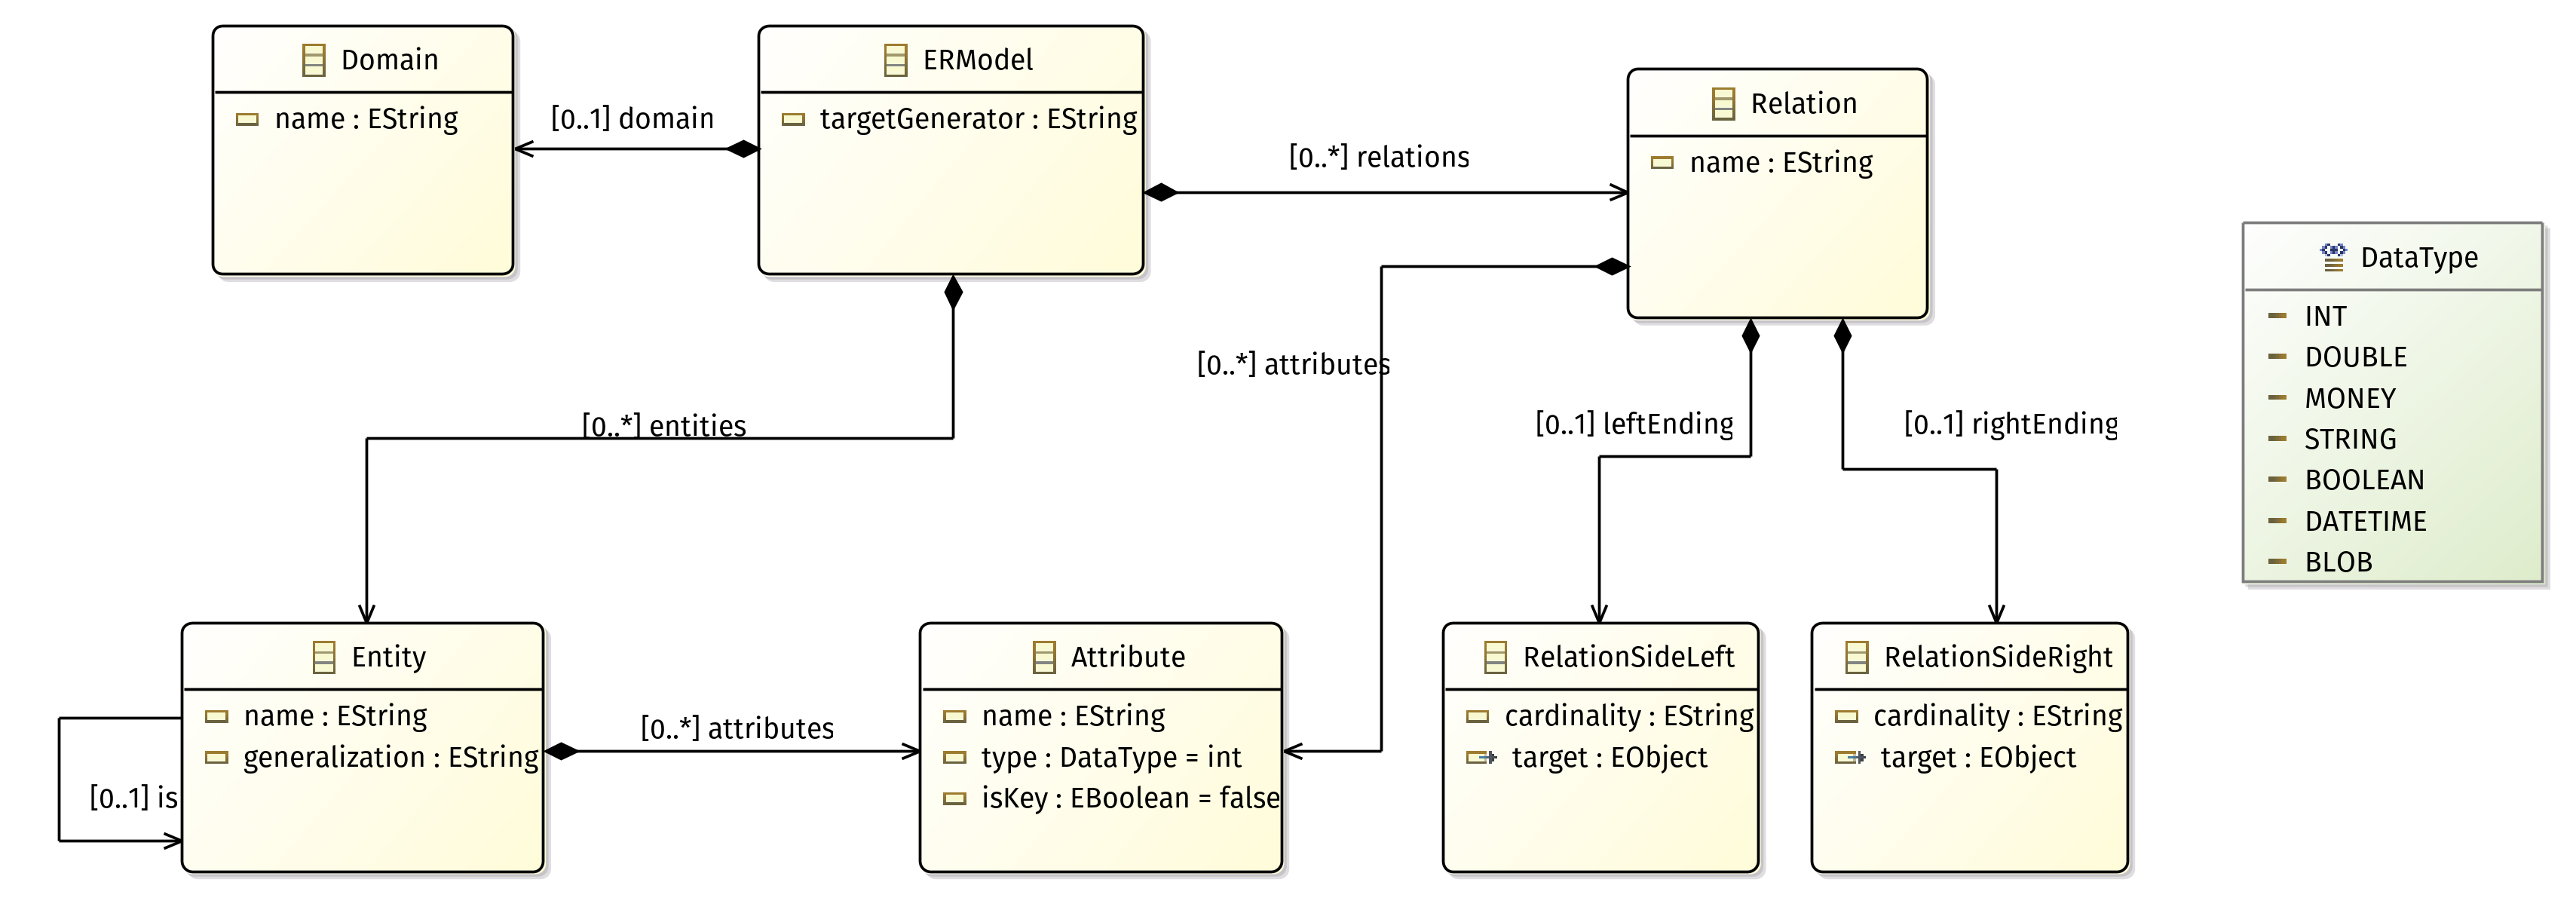
\includegraphics[width=\textwidth]{img/erDsl_class_diagram.png}
    \fonte{Author.}
\end{figure}

% O metamodelo da linguagem é importante na abordagem utilizada no Xtext pois permitiu que a DSL e os geradores sejam construídos separadamente. 
The language metamodel is relevant in the approach used in Xtext as it allowed the DSL and generators to be built separately.

%------------------------------------------------------------------------------
\subsection{Tool Architecture}
%------------------------------------------------------------------------------

% O framework Xtext gera grande parte da infraestrutura para linguagens com base fundamentalmente nas gramáticas definidas. 
% A Figura \ref{fig:arqXtext} fornece uma visão geral em um nível abstrato da arquitetura final da ERtext, arquitetura esta modificada com adição dos geradores SQL e gerador de diagramas com a PlantUML.
The Xtext framework generates much of the infrastructure for languages based fundamentally on defined grammar.
% FALAR DA ENGINE MWE2 ?
Figure \ref{fig:arqERtext} provides an abstract level overview of the final ERtext architecture, which we have modified by adding the SQL generators and diagram generator with PlantUML.
% Figure \ref{fig:arqERtext} provides an abstract level overview of the final ERtext architecture, which has been modified with the addition of SQL generators and diagram generator with PlantUML.

\begin{figure}[!htb]
    \centering
    \caption{ERtext architecture.}
    \label{fig:arqERtext}
    

\tikzset{every picture/.style={line width=0.75pt}} %set default line width to 0.75pt        

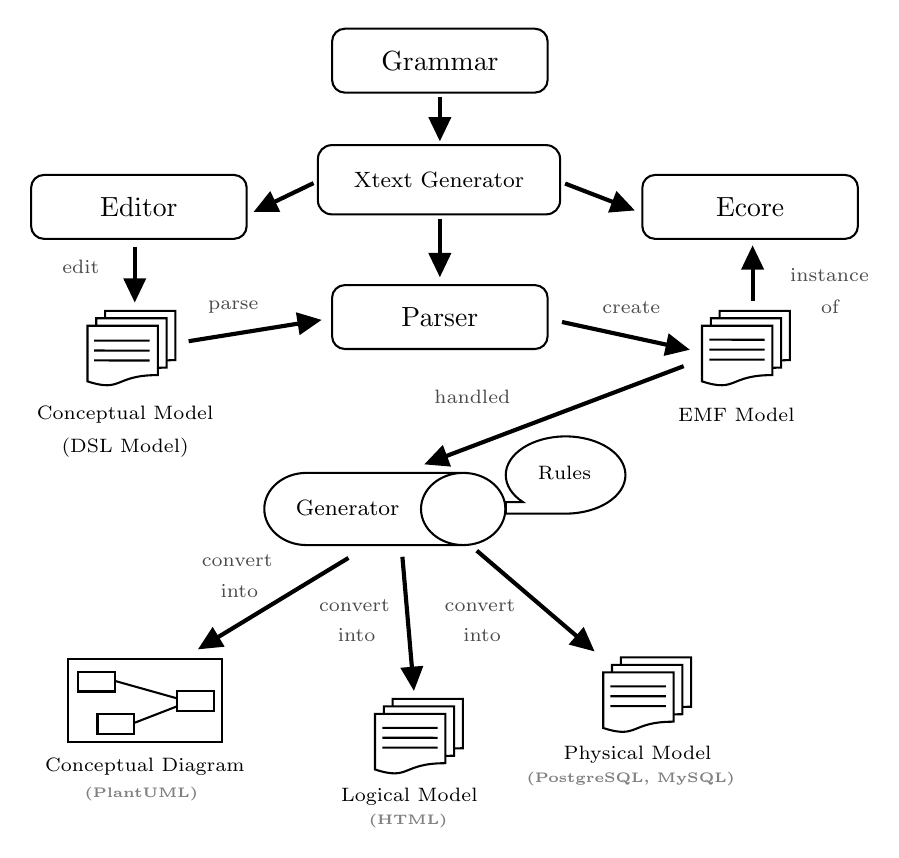
\begin{tikzpicture}[x=0.75pt,y=0.75pt,yscale=-1,xscale=1]
%uncomment if require: \path (0,465); %set diagram left start at 0, and has height of 465


%Rounded Rect [id:dp8080613887465731] 
\draw  [fill={rgb, 255:red, 255; green, 255; blue, 255 }  ,fill opacity=1 ] (268.24,22.37) .. controls (268.24,18.97) and (271,16.21) .. (274.4,16.21) -- (365.96,16.21) .. controls (369.36,16.21) and (372.11,18.97) .. (372.11,22.37) -- (372.11,40.84) .. controls (372.11,44.24) and (369.36,47) .. (365.96,47) -- (274.4,47) .. controls (271,47) and (268.24,44.24) .. (268.24,40.84) -- cycle ;
%Rounded Rect [id:dp23877247410758984] 
\draw  [fill={rgb, 255:red, 255; green, 255; blue, 255 }  ,fill opacity=1 ][line width=0.75]  (123.24,92.82) .. controls (123.24,89.42) and (126,86.66) .. (129.4,86.66) -- (220.95,86.66) .. controls (224.36,86.66) and (227.11,89.42) .. (227.11,92.82) -- (227.11,111.3) .. controls (227.11,114.7) and (224.36,117.46) .. (220.95,117.46) -- (129.4,117.46) .. controls (126,117.46) and (123.24,114.7) .. (123.24,111.3) -- cycle ;
%Flowchart: Multidocument [id:dp49717070559395604] 
\draw  [fill={rgb, 255:red, 255; green, 255; blue, 255 }  ,fill opacity=1 ] (158.88,152.12) -- (192.75,152.12) -- (192.75,175.89) .. controls (171.58,175.89) and (175.82,184.46) .. (158.88,178.91) -- cycle ; \draw  [fill={rgb, 255:red, 255; green, 255; blue, 255 }  ,fill opacity=1 ] (154.64,155.72) -- (188.52,155.72) -- (188.52,179.49) .. controls (167.35,179.49) and (171.58,188.06) .. (154.64,182.52) -- cycle ; \draw  [fill={rgb, 255:red, 255; green, 255; blue, 255 }  ,fill opacity=1 ] (150.41,159.32) -- (184.28,159.32) -- (184.28,183.09) .. controls (163.11,183.09) and (167.35,191.66) .. (150.41,186.12) -- cycle ;
%Straight Lines [id:da5642847406466045] 
\draw [fill={rgb, 255:red, 255; green, 255; blue, 255 }  ,fill opacity=1 ]   (153.63,166.47) -- (180.34,166.5) ;
%Straight Lines [id:da9779186616916171] 
\draw [fill={rgb, 255:red, 255; green, 255; blue, 255 }  ,fill opacity=1 ]   (153.63,171.26) -- (180.34,171.28) ;
%Straight Lines [id:da8217185402464098] 
\draw [fill={rgb, 255:red, 255; green, 255; blue, 255 }  ,fill opacity=1 ]   (153.63,176.04) -- (180.34,176.06) ;


%Straight Lines [id:da27204357118531197] 
\draw [fill={rgb, 255:red, 255; green, 255; blue, 255 }  ,fill opacity=1 ][line width=1.5]    (173.18,121.3) -- (173.18,144.06) ;
\draw [shift={(173.18,148.06)}, rotate = 270] [fill={rgb, 255:red, 0; green, 0; blue, 0 }  ][line width=0.08]  [draw opacity=0] (11.61,-5.58) -- (0,0) -- (11.61,5.58) -- cycle    ;
%Rounded Rect [id:dp014713549076222021] 
\draw  [fill={rgb, 255:red, 255; green, 255; blue, 255 }  ,fill opacity=1 ] (261.43,78.98) .. controls (261.43,75.3) and (264.41,72.31) .. (268.09,72.31) -- (371.45,72.31) .. controls (375.13,72.31) and (378.11,75.3) .. (378.11,78.98) -- (378.11,98.98) .. controls (378.11,102.66) and (375.13,105.65) .. (371.45,105.65) -- (268.09,105.65) .. controls (264.41,105.65) and (261.43,102.66) .. (261.43,98.98) -- cycle ;
%Rounded Rect [id:dp8159423215616721] 
\draw  [fill={rgb, 255:red, 255; green, 255; blue, 255 }  ,fill opacity=1 ] (417.72,92.82) .. controls (417.72,89.42) and (420.48,86.66) .. (423.88,86.66) -- (515.44,86.66) .. controls (518.84,86.66) and (521.59,89.42) .. (521.59,92.82) -- (521.59,111.3) .. controls (521.59,114.7) and (518.84,117.46) .. (515.44,117.46) -- (423.88,117.46) .. controls (420.48,117.46) and (417.72,114.7) .. (417.72,111.3) -- cycle ;
%Flowchart: Multidocument [id:dp814245162277164] 
\draw  [fill={rgb, 255:red, 255; green, 255; blue, 255 }  ,fill opacity=1 ] (454.96,152.12) -- (488.83,152.12) -- (488.83,175.89) .. controls (467.66,175.89) and (471.89,184.46) .. (454.96,178.91) -- cycle ; \draw  [fill={rgb, 255:red, 255; green, 255; blue, 255 }  ,fill opacity=1 ] (450.72,155.72) -- (484.6,155.72) -- (484.6,179.49) .. controls (463.43,179.49) and (467.66,188.06) .. (450.72,182.52) -- cycle ; \draw  [fill={rgb, 255:red, 255; green, 255; blue, 255 }  ,fill opacity=1 ] (446.49,159.32) -- (480.36,159.32) -- (480.36,183.09) .. controls (459.19,183.09) and (463.43,191.66) .. (446.49,186.12) -- cycle ;
%Straight Lines [id:da659202853659377] 
\draw [fill={rgb, 255:red, 255; green, 255; blue, 255 }  ,fill opacity=1 ]   (449.97,166.04) -- (476.69,166.06) ;
%Straight Lines [id:da8271632436642871] 
\draw [fill={rgb, 255:red, 255; green, 255; blue, 255 }  ,fill opacity=1 ]   (449.97,170.82) -- (476.69,170.85) ;
%Straight Lines [id:da22701123408508272] 
\draw [fill={rgb, 255:red, 255; green, 255; blue, 255 }  ,fill opacity=1 ]   (449.97,175.61) -- (476.69,175.63) ;


%Straight Lines [id:da6612735011438882] 
\draw [fill={rgb, 255:red, 255; green, 255; blue, 255 }  ,fill opacity=1 ][line width=1.5]    (470.86,124.65) -- (470.86,147.4) ;
\draw [shift={(470.86,120.65)}, rotate = 90] [fill={rgb, 255:red, 0; green, 0; blue, 0 }  ][line width=0.08]  [draw opacity=0] (11.61,-5.58) -- (0,0) -- (11.61,5.58) -- cycle    ;
%Rounded Rect [id:dp9641259565957541] 
\draw  [fill={rgb, 255:red, 255; green, 255; blue, 255 }  ,fill opacity=1 ] (268.24,145.89) .. controls (268.24,142.48) and (271,139.73) .. (274.4,139.73) -- (365.96,139.73) .. controls (369.36,139.73) and (372.11,142.48) .. (372.11,145.89) -- (372.11,164.36) .. controls (372.11,167.76) and (369.36,170.52) .. (365.96,170.52) -- (274.4,170.52) .. controls (271,170.52) and (268.24,167.76) .. (268.24,164.36) -- cycle ;
%Straight Lines [id:da4555835119587406] 
\draw [fill={rgb, 255:red, 255; green, 255; blue, 255 }  ,fill opacity=1 ][line width=1.5]    (320.18,48.89) -- (320.18,66.42) ;
\draw [shift={(320.18,70.42)}, rotate = 270] [fill={rgb, 255:red, 0; green, 0; blue, 0 }  ][line width=0.08]  [draw opacity=0] (11.61,-5.58) -- (0,0) -- (11.61,5.58) -- cycle    ;
%Straight Lines [id:da2586670416419199] 
\draw [fill={rgb, 255:red, 255; green, 255; blue, 255 }  ,fill opacity=1 ][line width=1.5]    (320.18,107.78) -- (320.18,131.88) ;
\draw [shift={(320.18,135.88)}, rotate = 270] [fill={rgb, 255:red, 0; green, 0; blue, 0 }  ][line width=0.08]  [draw opacity=0] (11.61,-5.58) -- (0,0) -- (11.61,5.58) -- cycle    ;
%Straight Lines [id:da2552674310073062] 
\draw [fill={rgb, 255:red, 255; green, 255; blue, 255 }  ,fill opacity=1 ][line width=1.5]    (259.32,90.59) -- (234.04,102.77) ;
\draw [shift={(230.43,104.51)}, rotate = 334.28] [fill={rgb, 255:red, 0; green, 0; blue, 0 }  ][line width=0.08]  [draw opacity=0] (11.61,-5.58) -- (0,0) -- (11.61,5.58) -- cycle    ;
%Straight Lines [id:da29550662771480396] 
\draw [fill={rgb, 255:red, 255; green, 255; blue, 255 }  ,fill opacity=1 ][line width=1.5]    (410.34,102.31) -- (380.52,90.81) ;
\draw [shift={(414.07,103.76)}, rotate = 201.11] [fill={rgb, 255:red, 0; green, 0; blue, 0 }  ][line width=0.08]  [draw opacity=0] (11.61,-5.58) -- (0,0) -- (11.61,5.58) -- cycle    ;
%Straight Lines [id:da3280771928101003] 
\draw [fill={rgb, 255:red, 255; green, 255; blue, 255 }  ,fill opacity=1 ][line width=1.5]    (199.15,166.77) -- (259.22,157.13) ;
\draw [shift={(263.17,156.5)}, rotate = 530.89] [fill={rgb, 255:red, 0; green, 0; blue, 0 }  ][line width=0.08]  [draw opacity=0] (11.61,-5.58) -- (0,0) -- (11.61,5.58) -- cycle    ;
%Straight Lines [id:da9478402467031726] 
\draw [fill={rgb, 255:red, 255; green, 255; blue, 255 }  ,fill opacity=1 ][line width=1.5]    (379.03,157.51) -- (436.63,170.02) ;
\draw [shift={(440.54,170.87)}, rotate = 192.26] [fill={rgb, 255:red, 0; green, 0; blue, 0 }  ][line width=0.08]  [draw opacity=0] (11.61,-5.58) -- (0,0) -- (11.61,5.58) -- cycle    ;
%Flowchart: Direct Access Storage [id:dp7657317583515377] 
\draw  [fill={rgb, 255:red, 255; green, 255; blue, 255 }  ,fill opacity=1 ] (331.43,264.99) -- (255.92,264.99) .. controls (244.69,264.99) and (235.59,257.2) .. (235.59,247.6) .. controls (235.59,238) and (244.69,230.21) .. (255.92,230.21) -- (331.43,230.21)(351.75,247.6) .. controls (351.75,257.2) and (342.65,264.99) .. (331.43,264.99) .. controls (320.2,264.99) and (311.1,257.2) .. (311.1,247.6) .. controls (311.1,238) and (320.2,230.21) .. (331.43,230.21) .. controls (342.65,230.21) and (351.75,238) .. (351.75,247.6) ;
%Straight Lines [id:da100480350897858] 
\draw [fill={rgb, 255:red, 255; green, 255; blue, 255 }  ,fill opacity=1 ][line width=1.5]    (437.65,178.79) -- (316.46,224.67) ;
\draw [shift={(312.72,226.08)}, rotate = 339.27] [fill={rgb, 255:red, 0; green, 0; blue, 0 }  ][line width=0.08]  [draw opacity=0] (11.61,-5.58) -- (0,0) -- (11.61,5.58) -- cycle    ;
%Flowchart: Multidocument [id:dp5253239734010293] 
\draw  [fill={rgb, 255:red, 255; green, 255; blue, 255 }  ,fill opacity=1 ] (297.41,339.12) -- (331.29,339.12) -- (331.29,362.88) .. controls (310.11,362.88) and (314.35,371.45) .. (297.41,365.91) -- cycle ; \draw  [fill={rgb, 255:red, 255; green, 255; blue, 255 }  ,fill opacity=1 ] (293.18,342.72) -- (327.05,342.72) -- (327.05,366.48) .. controls (305.88,366.48) and (310.11,375.05) .. (293.18,369.51) -- cycle ; \draw  [fill={rgb, 255:red, 255; green, 255; blue, 255 }  ,fill opacity=1 ] (288.94,346.32) -- (322.82,346.32) -- (322.82,370.08) .. controls (301.65,370.08) and (305.88,378.66) .. (288.94,373.11) -- cycle ;
%Straight Lines [id:da29635223798470123] 
\draw [fill={rgb, 255:red, 255; green, 255; blue, 255 }  ,fill opacity=1 ]   (292.43,353.03) -- (319.14,353.05) ;
%Straight Lines [id:da45709195099870326] 
\draw [fill={rgb, 255:red, 255; green, 255; blue, 255 }  ,fill opacity=1 ]   (292.43,357.82) -- (319.14,357.84) ;
%Straight Lines [id:da9397926099052756] 
\draw [fill={rgb, 255:red, 255; green, 255; blue, 255 }  ,fill opacity=1 ]   (292.43,362.6) -- (319.14,362.62) ;




%Straight Lines [id:da10826901476686546] 
\draw [fill={rgb, 255:red, 255; green, 255; blue, 255 }  ,fill opacity=1 ][line width=1.5]    (302.13,270.64) -- (307.34,331.21) ;
\draw [shift={(307.68,335.2)}, rotate = 265.08] [fill={rgb, 255:red, 0; green, 0; blue, 0 }  ][line width=0.08]  [draw opacity=0] (11.61,-5.58) -- (0,0) -- (11.61,5.58) -- cycle    ;
%Flowchart: Sequential Access Storage [id:dp3007368871754543] 
\draw  [fill={rgb, 255:red, 255; green, 255; blue, 255 }  ,fill opacity=1 ] (409.6,231.24) .. controls (409.6,220.96) and (396.69,212.63) .. (380.76,212.63) .. controls (364.84,212.63) and (351.93,220.96) .. (351.93,231.24) .. controls (351.93,236.31) and (355.07,240.9) .. (360.17,244.26) -- (351.93,244.26) -- (351.93,249.84) -- (380.76,249.84) .. controls (396.69,249.84) and (409.6,241.51) .. (409.6,231.24) -- cycle ;
%Shape: Rectangle [id:dp03278310257286665] 
\draw   (141.03,319.87) -- (215.03,319.87) -- (215.03,359.87) -- (141.03,359.87) -- cycle ;
%Shape: Rectangle [id:dp9445861445312367] 
\draw   (145.83,326.14) -- (163.55,326.14) -- (163.55,335.52) -- (145.83,335.52) -- cycle ;
%Shape: Rectangle [id:dp035309426832852875] 
\draw   (193.63,335.34) -- (211.34,335.34) -- (211.34,344.72) -- (193.63,344.72) -- cycle ;
%Shape: Rectangle [id:dp0682098761538128] 
\draw   (155.23,346.54) -- (172.94,346.54) -- (172.94,355.92) -- (155.23,355.92) -- cycle ;
%Straight Lines [id:da09626722375251995] 
\draw    (172.65,350.78) -- (193.32,342.78) ;
%Straight Lines [id:da41470258123307224] 
\draw    (163.65,330.44) -- (193.32,338.78) ;


%Straight Lines [id:da24414024149042923] 
\draw [fill={rgb, 255:red, 255; green, 255; blue, 255 }  ,fill opacity=1 ][line width=1.5]    (276.13,271.19) -- (207.1,313.12) ;
\draw [shift={(203.68,315.2)}, rotate = 328.72] [fill={rgb, 255:red, 0; green, 0; blue, 0 }  ][line width=0.08]  [draw opacity=0] (11.61,-5.58) -- (0,0) -- (11.61,5.58) -- cycle    ;
%Flowchart: Multidocument [id:dp9410827405643849] 
\draw  [fill={rgb, 255:red, 255; green, 255; blue, 255 }  ,fill opacity=1 ] (407.36,319.12) -- (441.24,319.12) -- (441.24,342.88) .. controls (420.07,342.88) and (424.3,351.45) .. (407.36,345.91) -- cycle ; \draw  [fill={rgb, 255:red, 255; green, 255; blue, 255 }  ,fill opacity=1 ] (403.13,322.72) -- (437.01,322.72) -- (437.01,346.48) .. controls (415.83,346.48) and (420.07,355.05) .. (403.13,349.51) -- cycle ; \draw  [fill={rgb, 255:red, 255; green, 255; blue, 255 }  ,fill opacity=1 ] (398.89,326.32) -- (432.77,326.32) -- (432.77,350.08) .. controls (411.6,350.08) and (415.83,358.66) .. (398.89,353.11) -- cycle ;
%Straight Lines [id:da31801059922861796] 
\draw [fill={rgb, 255:red, 255; green, 255; blue, 255 }  ,fill opacity=1 ]   (402.38,333.03) -- (429.1,333.05) ;
%Straight Lines [id:da19940799584772861] 
\draw [fill={rgb, 255:red, 255; green, 255; blue, 255 }  ,fill opacity=1 ]   (402.38,337.82) -- (429.1,337.84) ;
%Straight Lines [id:da720164043002747] 
\draw [fill={rgb, 255:red, 255; green, 255; blue, 255 }  ,fill opacity=1 ]   (402.38,342.6) -- (429.1,342.62) ;




%Straight Lines [id:da4341747356667731] 
\draw [fill={rgb, 255:red, 255; green, 255; blue, 255 }  ,fill opacity=1 ][line width=1.5]    (337.96,267.69) -- (391.64,313.6) ;
\draw [shift={(394.68,316.2)}, rotate = 220.53] [fill={rgb, 255:red, 0; green, 0; blue, 0 }  ][line width=0.08]  [draw opacity=0] (11.61,-5.58) -- (0,0) -- (11.61,5.58) -- cycle    ;



% Text Node
\draw (175.18,102.06) node   [align=left] {Editor};
% Text Node
\draw (469.66,102.06) node   [align=left] {Ecore};
% Text Node
\draw (320.18,155.12) node   [align=left] {Parser};
% Text Node
\draw (320.18,31.6) node  [font=\normalsize] [align=left] {Grammar};
% Text Node
\draw (168.54,201.99) node   [align=left] {{\scriptsize Conceptual Model}};
% Text Node
\draw (463.03,201.99) node   [align=left] {{\scriptsize EMF Model}};
% Text Node
\draw (275.76,247.14) node  [font=\footnotesize] [align=left] {\begin{minipage}[lt]{39.43pt}\setlength\topsep{0pt}
\begin{center}
Generator
\end{center}

\end{minipage}};
% Text Node
\draw (380.24,230.37) node  [font=\scriptsize] [align=left] {\begin{minipage}[lt]{20.96pt}\setlength\topsep{0pt}
\begin{center}
Rules
\end{center}

\end{minipage}};
% Text Node
\draw (136.8,126.16) node [anchor=north west][inner sep=0.75pt]  [font=\scriptsize,color={rgb, 255:red, 74; green, 74; blue, 74 }  ,opacity=1 ] [align=left] {edit};
% Text Node
\draw (207,146.18) node [anchor=north west][inner sep=0.75pt]  [font=\scriptsize,color={rgb, 255:red, 74; green, 74; blue, 74 }  ,opacity=1 ] [align=left] {parse};
% Text Node
\draw (397,146.18) node [anchor=north west][inner sep=0.75pt]  [font=\scriptsize,color={rgb, 255:red, 74; green, 74; blue, 74 }  ,opacity=1 ] [align=left] {create};
% Text Node
\draw (487.4,130.21) node [anchor=north west][inner sep=0.75pt]  [font=\scriptsize,color={rgb, 255:red, 74; green, 74; blue, 74 }  ,opacity=1 ] [align=left] {instance};
% Text Node
\draw (316,188.69) node [anchor=north west][inner sep=0.75pt]  [font=\scriptsize,color={rgb, 255:red, 74; green, 74; blue, 74 }  ,opacity=1 ] [align=left] {handled};
% Text Node
\draw (502.4,145.21) node [anchor=north west][inner sep=0.75pt]  [font=\scriptsize,color={rgb, 255:red, 74; green, 74; blue, 74 }  ,opacity=1 ] [align=left] {of};
% Text Node
\draw (319.77,88.98) node  [font=\footnotesize] [align=left] {Xtext Generator};
% Text Node
\draw (168.54,217.99) node   [align=left] {{\scriptsize (DSL Model)}};
% Text Node
\draw (204,268.3) node [anchor=north west][inner sep=0.75pt]  [font=\scriptsize,color={rgb, 255:red, 74; green, 74; blue, 74 }  ,opacity=1 ] [align=left] {convert};
% Text Node
\draw (213,282.3) node [anchor=north west][inner sep=0.75pt]  [font=\scriptsize,color={rgb, 255:red, 74; green, 74; blue, 74 }  ,opacity=1 ] [align=left] {into};
% Text Node
\draw (305.48,385.98) node   [align=left] {{\scriptsize Logical Model}};
% Text Node
\draw (415.43,365.98) node   [align=left] {{\scriptsize Physical Model}};
% Text Node
\draw (284.48,392.91) node [anchor=north west][inner sep=0.75pt]   [align=left] {{\tiny \textcolor[rgb]{0.5,0.5,0.5}{\textbf{(HTML)}}}};
% Text Node
\draw (360.43,372.91) node [anchor=north west][inner sep=0.75pt]   [align=left] {{\tiny \textcolor[rgb]{0.5,0.5,0.5}{\textbf{(PostgreSQL, MySQL)}}}};
% Text Node
\draw (147.53,380.15) node [anchor=north west][inner sep=0.75pt]   [align=left] {{\tiny \textcolor[rgb]{0.5,0.5,0.5}{\textbf{(PlantUML)}}}};
% Text Node
\draw (178.03,371.89) node   [align=left] {{\scriptsize Conceptual Diagram}};
% Text Node
\draw (269.5,303.8) node [anchor=north west][inner sep=0.75pt]  [font=\scriptsize,color={rgb, 255:red, 74; green, 74; blue, 74 }  ,opacity=1 ] [align=left] {into};
% Text Node
\draw (260.5,289.8) node [anchor=north west][inner sep=0.75pt]  [font=\scriptsize,color={rgb, 255:red, 74; green, 74; blue, 74 }  ,opacity=1 ] [align=left] {convert};
% Text Node
\draw (330,303.8) node [anchor=north west][inner sep=0.75pt]  [font=\scriptsize,color={rgb, 255:red, 74; green, 74; blue, 74 }  ,opacity=1 ] [align=left] {into};
% Text Node
\draw (321,289.8) node [anchor=north west][inner sep=0.75pt]  [font=\scriptsize,color={rgb, 255:red, 74; green, 74; blue, 74 }  ,opacity=1 ] [align=left] {convert};


\end{tikzpicture}

    \fonte{Author.}
\end{figure}

% Dizemos que o Xtext gera grande parte, e não completamente, pois existem diversos aspectos que devem ser implementados de acordo com os requisitos e objetivos da linguagem.
% Por exemplo, toda a parte de validação com com base no escopo, marcação e feedback de erros, sugestão de trechos de código, criação de templates, e wizards de criação de projetos e arquivos específicos para a linguagem precisam e foram implementados manualmente.
We say that Xtext generates a majority part, but not entirely, as several aspects must be implemented according to the requirements and objectives of the language.
% For example, all of the scope-based validation, bug marking and feedback, snippet suggestion, template creation, and language-specific project and file creation wizards need and have been implemented manually.
For example, we have manually needed and implemented the following aspects, all of the scope-based validation, bug marking and feedback, snippet suggestion, template creation, and language-specific project and file creation wizards.

%------------------------------------------------------------------------------
\subsection{Stable Version}
%------------------------------------------------------------------------------

% O código fonte da versão estável da ferramenta de modelagem produzida está disponível em um repositório público no GitHub\footnote{Repositório: \url{https://github.com/ProjetoDSL/ERDSL}}.
% Esta versão será irá para a última avaliação experimental que será planejada para avaliar não só a \ac{dsl} como também os artefatos que podem ser produzidos por ela, bem como sua usabilidade.
% A Figura \ref{fig:stableVersion} apresenta um fragmento visual da ferramenta em uso.
The source code of the stable version of the produced modeling tool is available in a public repository on GitHub\footnote{Repository: \url{https://github.com/ProjetoDSL/ERDSL}}.
This version gone to the last experimental evaluation which was designed to evaluate not only the \ac{dsl} but also the artifacts that can be produced by it, as well as its usability.
Figure \ref{fig:stableVersion} presents a visual fragment of the tool in use.

\begin{figure} [!htb]
    \centering
    \caption{ERtext tool stable version.}
    \label{fig:stableVersion}
    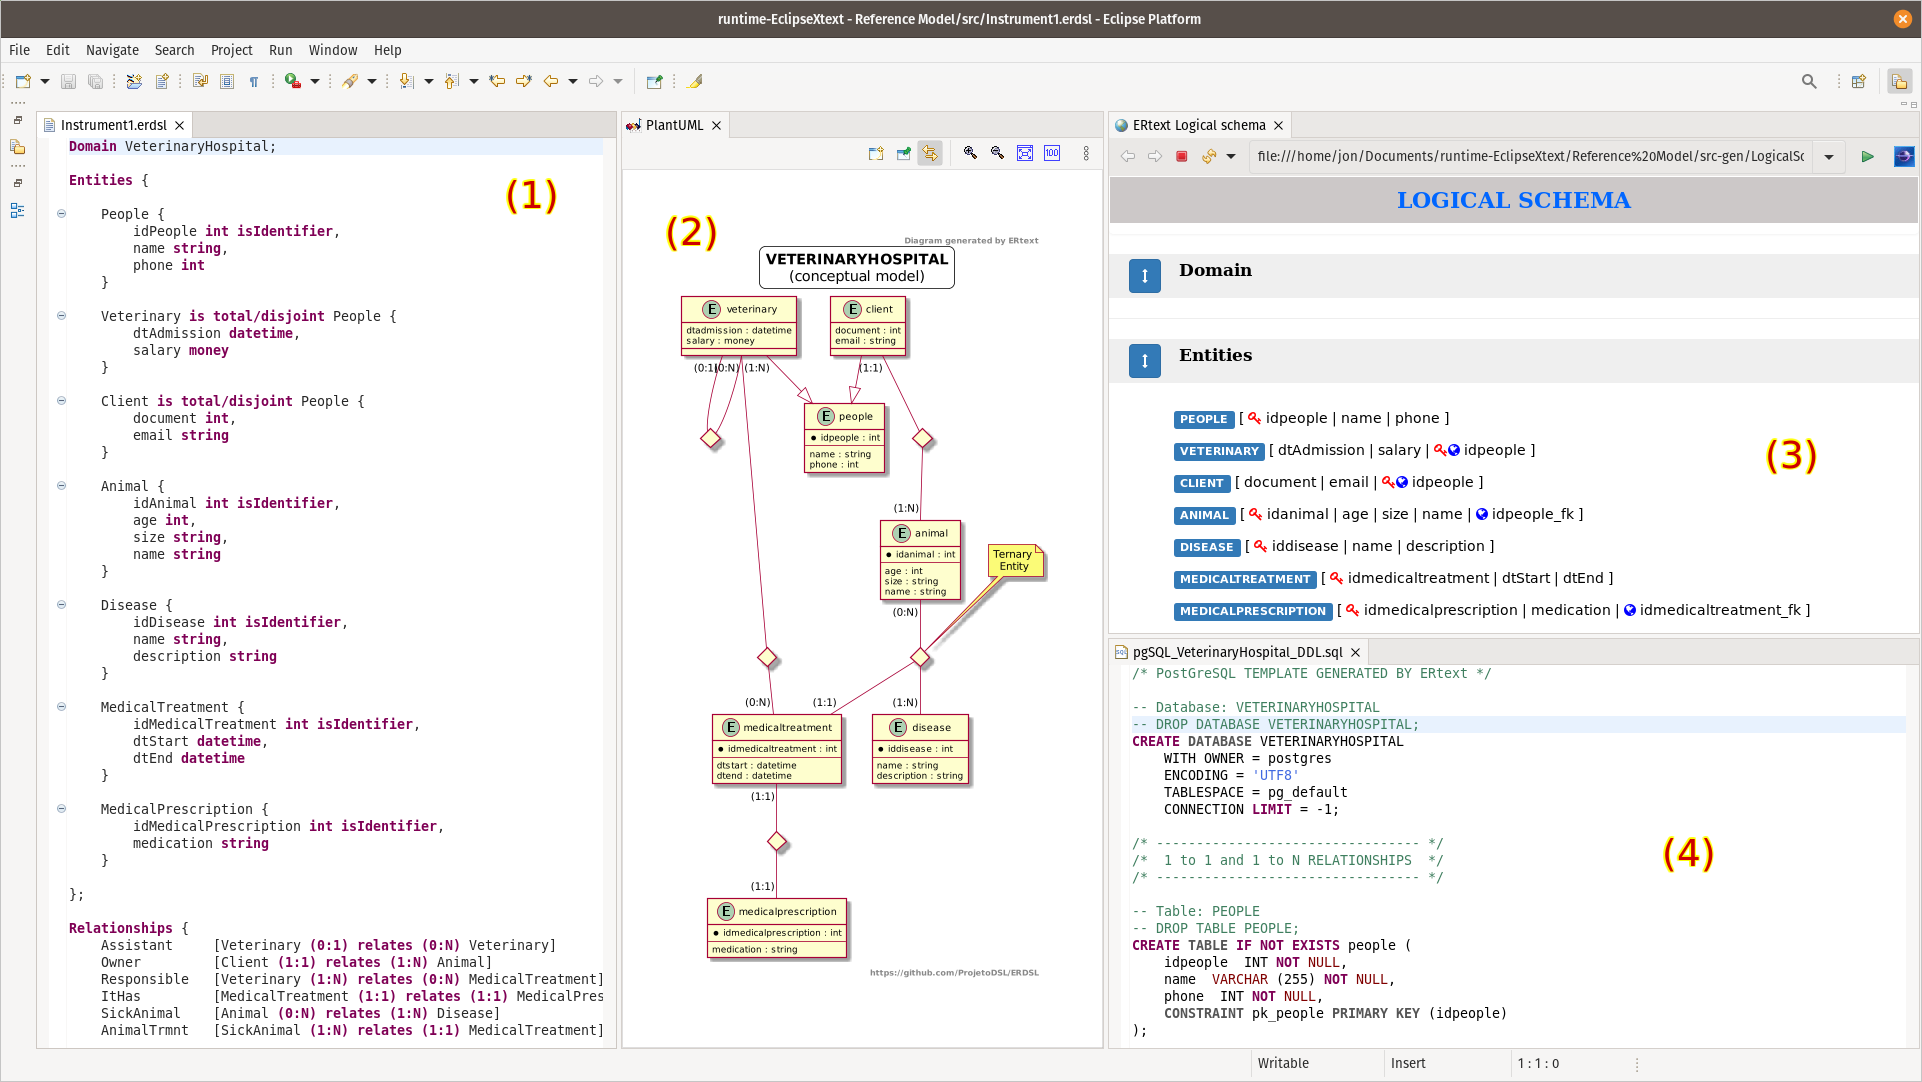
\includegraphics[width=1\textwidth]{img/ToolOverview2.png}
    \fonte{Author.}
\end{figure}

% A legenda (1) na figura demonstra o editor com um modelo descrito na DSL implementada. A legenda (2) apresenta uma representação gráfica (diagrama) utilizando a integração com PlantUML. 
% Para isto o modelo é transformado da nossa DSL para a notação necessária para o PlantUML gerar o diagrama utilizando bibliotecas do Graphviz.
% A legenda (3) mostra o modelo transformado para uma notação lógica, já resolvendo as relações, ou seja, as chaves primárias e estrangeiras.
% Finalmente, na legenda (4) apresentamos o código SQL DDL gerada para o \ac{dbms} PostgreSQL 
The caption (1) in the figure demonstrates the editor with a model described in the implemented \ac{dsl} notation.
Caption (2) presents a graphical representation (diagram) using the integration with PlantUML.
For this, the model is transformed from our \ac{dsl} to the necessary notation for PlantUML to generate the diagram using Graphviz libraries.
Caption (3) shows the model transformed to a logical notation, already solving the relations, \textit{i.e.} the primary and foreign keys.
Finally, in caption (4) we present the generated \ac{sql} \ac{ddl} code for \ac{dbms} PostgreSQL.

% Para as tranformações dos modelos foi avaliado as opções de regras de transformações descritas por~\cite{Heuser:2009}.
% Em relação aos relacionamentos do tipo 1:1 adotou-se a estratégia de adição de coluna para os três casos possíveis.
% Para os relacionamentos 1:N seguiu-se a mesma premissa de transformação para os quatro (4) casos possíveis.
% Já para a transformação de relacionamentos N:N optou-se pela única regra de transformação recomendada, ou seja, a regra de criação de tabelas próprias para os três (3) casos.
For the transformations of the models, we have evaluated the transformation rule options described by~\cite{Heuser:2009}.
Regarding 1:1 type relationships, we have adopted the column addition strategy for the three (3) possible cases.
For the 1:N relationships, we have followed the same transformation premise for the four (4) possible cases.
For the transformation of N:N relationships, we have chosen the only recommended transformation rule, \textit{i.e.} the rule for creating own tables for the three (3) cases.

% Basicamente durante a atividade de modelagem um arquivo de texto plano é criado com a extensão da linguagem (.erdsl) no sistema que está rodando a ferramenta.
% A cada vez que este arquivo é salvo um modelo Ecore é criado ou atualizado para então ser chamado aos geradores que lidam com os artefatos que devem ser criados.
% Isto acontece através da interface \ texttt {IFileSystemAccess2} que oferece o meio para percorrer o modelo criado e aplicar como regras de transformação em um cenário standalone.
% Esta interface oferece uma abstração para operações no sistema de arquivos, possibilitando o mapeamento de caminho lógico (artefato de saída). 
% Esta interface compõe todas as interfaces de extensão para \ texttt {IFileSystemAccess} com outras melhorias implementadas diretamente.
Basically, during the modeling activity a plain text file is created with the language extension (.erdsl) on the system running the tool.
Each time this file is saved, an Ecore model is created or updated and then called to the generators that handle the artifacts that must be created.
It happens through the \texttt {IFileSystemAccess2} interface that provides the means to iterate through the created model and apply as transformation rules in a standalone scenario.
This interface provides an abstraction for file system operations, enabling logical path mapping (output artifact).
This interface composes all the extension interfaces for \texttt {IFileSystemAccess} with other improvements implemented.

% Para registro, nossos geradores especializados utilizam o padrão de projeto Template Method na sua implementação.
% O Template Method é um padrão de projeto comportamental, que define o esqueleto de um algoritmo em uma superclasse, deixando as subclasses sobrescreverem etapas específicas do algoritmo sem modificar sua estrutura.
For the sake of the record, our specialized generators use the Template Method design pattern~\cite{GOF:95} in their implementation.
% For the record, our specialized generators use the Template Method design pattern~\cite{GOF:95} in their implementation.
The Template Method is a behavioral design pattern that defines a structure of an algorithm in a superclass, letting the subclasses override specific steps of the algorithm without modifying its structure.

% Este padrão de projeto preconiza que o algoritmo precisa ser modularizado em uma série de etapas, transformando essas etapas em métodos, e colocando uma série de chamadas para esses métodos dentro de um único método padrão. 
% Em nossa solução as etapas dessa tranformação são definidas em uma classe abstrata. 
% Desta forma nossos geradores especializados implementam todas estas etapas abstratas, e eventualmente sobrescrevem algumas das opcionais quando necessário, mas nunca o próprio método padrão.
This design pattern recommends that the algorithm be modularized into a series of steps, transforming these steps into methods and placing a series of calls to these methods within a single default method.
% This design pattern recommends that the algorithm needs to be modularized into a series of steps, transforming these steps into methods and placing a series of calls to these methods within a single standard method.
In our solution, we defined the steps of this transformation in an abstract class.
% In our solution the steps of this transformation are defined in an abstract class.
Thus, our specialized generators implement all these abstract steps and eventually override some optional ones when necessary, but never the default method itself.

% \begin{figure}[!htb]
%     \centering
%     \caption{Transformation rules adopted.}
%     \label{fig:transformationRules}
%     

\tikzset{every picture/.style={line width=0.75pt}} %set default line width to 0.75pt        

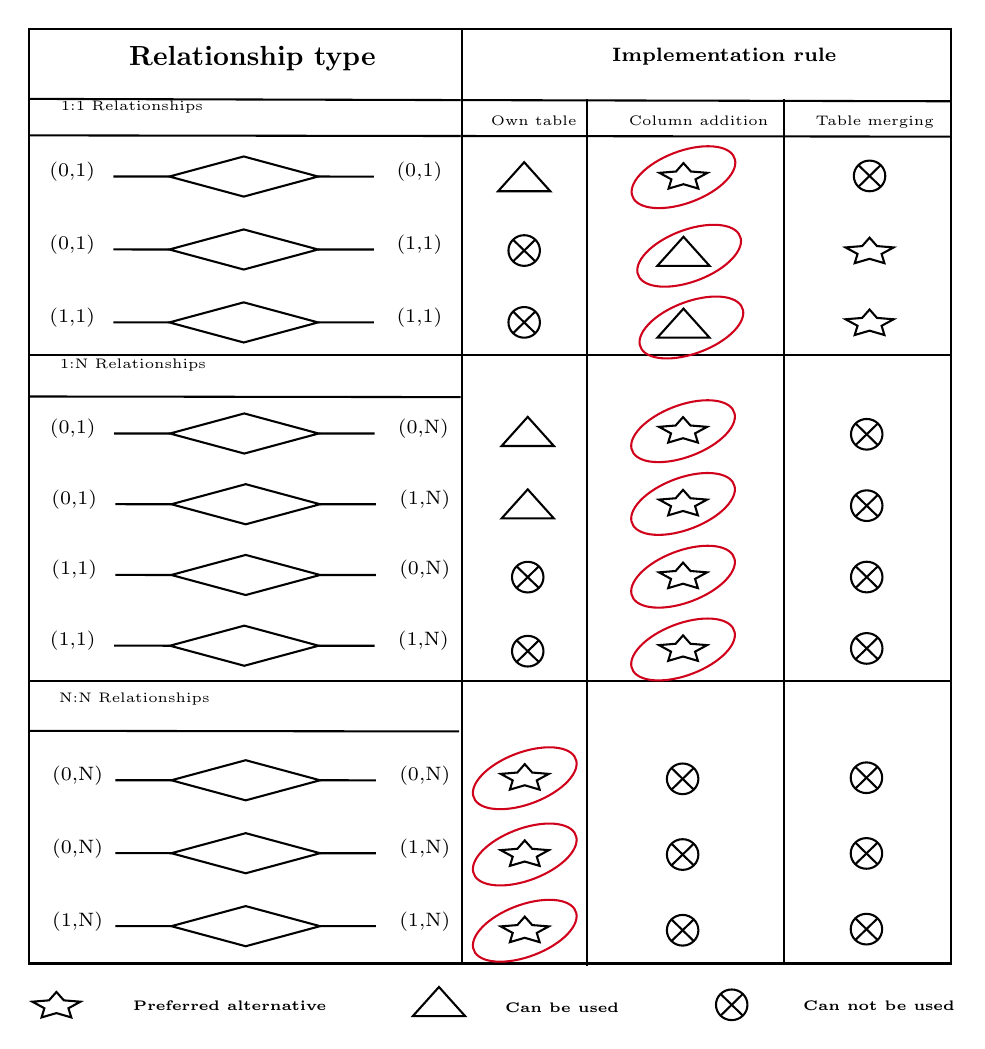
\begin{tikzpicture}[x=0.75pt,y=0.75pt,yscale=-1,xscale=1]
%uncomment if require: \path (0,499); %set diagram left start at 0, and has height of 499

%Shape: Star [id:dp905069961258552] 
\draw   (18.05,469.49) -- (21.63,473.53) -- (29.64,474.18) -- (23.84,477.33) -- (25.21,481.76) -- (18.05,479.67) -- (10.88,481.76) -- (12.25,477.33) -- (6.46,474.18) -- (14.47,473.53) -- cycle ;
%Flowchart: Summing Junction [id:dp5670844386539957] 
\draw   (335.82,475.68) .. controls (335.82,471.6) and (339.21,468.29) .. (343.4,468.29) .. controls (347.59,468.29) and (350.98,471.6) .. (350.98,475.68) .. controls (350.98,479.75) and (347.59,483.06) .. (343.4,483.06) .. controls (339.21,483.06) and (335.82,479.75) .. (335.82,475.68) -- cycle ; \draw   (338.04,470.45) -- (348.76,480.9) ; \draw   (348.76,470.45) -- (338.04,480.9) ;
%Shape: Triangle [id:dp8755221528505448] 
\draw   (202.36,467.09) -- (214.95,481.1) -- (189.78,481.1) -- cycle ;
%Shape: Diamond [id:dp15610691613574645] 
\draw   (108.29,66.95) -- (144.12,76.62) -- (108.29,86.29) -- (72.46,76.62) -- cycle ;
%Straight Lines [id:da1548262316328981] 
\draw    (72.46,76.62) -- (45.55,76.61) ;
%Straight Lines [id:da34976069343568916] 
\draw    (171.03,76.63) -- (144.12,76.62) ;


%Shape: Rectangle [id:dp9438218872468358] 
\draw   (4.84,5.4) -- (213.33,5.4) -- (213.33,162.47) -- (4.84,162.47) -- cycle ;
%Shape: Diamond [id:dp2599956034792046] 
\draw   (108.29,102.1) -- (144.12,111.77) -- (108.29,121.43) -- (72.46,111.77) -- cycle ;
%Straight Lines [id:da5197763190540488] 
\draw    (72.46,111.77) -- (45.55,111.75) ;
%Straight Lines [id:da8940402532777019] 
\draw    (171.03,111.78) -- (144.12,111.77) ;


%Shape: Diamond [id:dp7953044653471437] 
\draw   (108.29,137.24) -- (144.12,146.91) -- (108.29,156.58) -- (72.46,146.91) -- cycle ;
%Straight Lines [id:da20949304709496497] 
\draw    (72.46,146.91) -- (45.55,146.9) ;
%Straight Lines [id:da34589572563098536] 
\draw    (171.03,146.92) -- (144.12,146.91) ;


%Straight Lines [id:da22563177204480978] 
\draw    (5.11,39.21) -- (212.78,39.79) ;
%Straight Lines [id:da6727878622034686] 
\draw    (5.38,56.79) -- (212.78,57.1) ;
%Straight Lines [id:da03418802907814289] 
\draw    (212.78,57.1) -- (448.88,57.4) ;
%Straight Lines [id:da9489243894366923] 
\draw    (212.78,39.79) -- (449.15,40.36) ;
%Shape: Rectangle [id:dp7744485792611493] 
\draw   (213.33,5.4) -- (449.14,5.4) -- (449.14,162.47) -- (213.33,162.47) -- cycle ;
%Straight Lines [id:da1104964129518442] 
\draw    (273.52,39.45) -- (273.52,162.59) ;
%Straight Lines [id:da5208240902682426] 
\draw    (368.51,39.09) -- (368.51,162.23) ;
%Shape: Star [id:dp5079293847310995] 
\draw   (319.96,192.53) -- (323.54,196.57) -- (331.55,197.22) -- (325.75,200.36) -- (327.12,204.8) -- (319.96,202.7) -- (312.8,204.8) -- (314.16,200.36) -- (308.37,197.22) -- (316.38,196.57) -- cycle ;
%Shape: Triangle [id:dp4199850954698714] 
\draw   (245.13,192.42) -- (257.72,206.43) -- (232.54,206.43) -- cycle ;
%Flowchart: Summing Junction [id:dp2114922561352448] 
\draw   (400.87,200.8) .. controls (400.87,196.72) and (404.27,193.42) .. (408.45,193.42) .. controls (412.64,193.42) and (416.04,196.72) .. (416.04,200.8) .. controls (416.04,204.88) and (412.64,208.19) .. (408.45,208.19) .. controls (404.27,208.19) and (400.87,204.88) .. (400.87,200.8) -- cycle ; \draw   (403.09,195.58) -- (413.82,206.02) ; \draw   (413.82,195.58) -- (403.09,206.02) ;
%Shape: Star [id:dp051836092901429875] 
\draw   (320.16,70.15) -- (323.74,74.19) -- (331.75,74.84) -- (325.95,77.98) -- (327.32,82.42) -- (320.16,80.32) -- (312.99,82.42) -- (314.36,77.98) -- (308.57,74.84) -- (316.58,74.19) -- cycle ;
%Shape: Triangle [id:dp16503862399573688] 
\draw   (320.16,105.65) -- (332.74,119.66) -- (307.57,119.66) -- cycle ;
%Shape: Triangle [id:dp2109056154155149] 
\draw   (320.16,140.26) -- (332.74,154.27) -- (307.57,154.27) -- cycle ;
%Shape: Triangle [id:dp6106295252529019] 
\draw   (243.42,69.71) -- (256.01,83.72) -- (230.84,83.72) -- cycle ;
%Flowchart: Summing Junction [id:dp7641214677961137] 
\draw   (235.84,112.27) .. controls (235.84,108.19) and (239.23,104.89) .. (243.42,104.89) .. controls (247.61,104.89) and (251,108.19) .. (251,112.27) .. controls (251,116.35) and (247.61,119.66) .. (243.42,119.66) .. controls (239.23,119.66) and (235.84,116.35) .. (235.84,112.27) -- cycle ; \draw   (238.06,107.05) -- (248.78,117.5) ; \draw   (248.78,107.05) -- (238.06,117.5) ;
%Flowchart: Summing Junction [id:dp22623131635410432] 
\draw   (235.84,146.89) .. controls (235.84,142.81) and (239.23,139.5) .. (243.42,139.5) .. controls (247.61,139.5) and (251,142.81) .. (251,146.89) .. controls (251,150.96) and (247.61,154.27) .. (243.42,154.27) .. controls (239.23,154.27) and (235.84,150.96) .. (235.84,146.89) -- cycle ; \draw   (238.06,141.66) -- (248.78,152.11) ; \draw   (248.78,141.66) -- (238.06,152.11) ;
%Flowchart: Summing Junction [id:dp8111950400823971] 
\draw   (402.24,76.33) .. controls (402.24,72.25) and (405.63,68.94) .. (409.82,68.94) .. controls (414.01,68.94) and (417.4,72.25) .. (417.4,76.33) .. controls (417.4,80.41) and (414.01,83.72) .. (409.82,83.72) .. controls (405.63,83.72) and (402.24,80.41) .. (402.24,76.33) -- cycle ; \draw   (404.46,71.11) -- (415.18,81.55) ; \draw   (415.18,71.11) -- (404.46,81.55) ;
%Shape: Star [id:dp8714716991158269] 
\draw   (409.82,106.09) -- (413.4,110.13) -- (421.41,110.78) -- (415.62,113.92) -- (416.98,118.36) -- (409.82,116.27) -- (402.66,118.36) -- (404.03,113.92) -- (398.23,110.78) -- (406.24,110.13) -- cycle ;
%Shape: Star [id:dp9624342328821995] 
\draw   (409.82,140.7) -- (413.4,144.74) -- (421.41,145.39) -- (415.62,148.54) -- (416.98,152.98) -- (409.82,150.88) -- (402.66,152.98) -- (404.03,148.54) -- (398.23,145.39) -- (406.24,144.74) -- cycle ;
%Shape: Rectangle [id:dp04619740593055166] 
\draw   (4.84,162.47) -- (213.33,162.47) -- (213.33,319.53) -- (4.84,319.53) -- cycle ;
%Shape: Diamond [id:dp27789691615521184] 
\draw   (108.57,190.76) -- (144.39,200.43) -- (108.57,210.09) -- (72.74,200.43) -- cycle ;
%Straight Lines [id:da6441724439769754] 
\draw    (72.74,200.43) -- (45.83,200.41) ;
%Straight Lines [id:da38653260527553623] 
\draw    (171.31,200.44) -- (144.39,200.43) ;


%Shape: Diamond [id:dp2739495911529186] 
\draw   (109.25,224.84) -- (145.08,234.51) -- (109.25,244.17) -- (73.42,234.51) -- cycle ;
%Straight Lines [id:da7680368197813587] 
\draw    (73.42,234.51) -- (46.51,234.49) ;
%Straight Lines [id:da16254742962238433] 
\draw    (171.99,234.52) -- (145.08,234.51) ;


%Shape: Diamond [id:dp37713417833040097] 
\draw   (109.25,258.92) -- (145.08,268.59) -- (109.25,278.25) -- (73.42,268.59) -- cycle ;
%Straight Lines [id:da7776121131254392] 
\draw    (73.42,268.59) -- (46.51,268.57) ;
%Straight Lines [id:da010163980070524659] 
\draw    (171.99,268.6) -- (145.08,268.59) ;


%Straight Lines [id:da17800868812349258] 
\draw    (5.38,182.59) -- (212.78,182.9) ;
%Shape: Diamond [id:dp5731700485298001] 
\draw   (108.57,293) -- (144.39,302.67) -- (108.57,312.33) -- (72.74,302.67) -- cycle ;
%Straight Lines [id:da44119921508225857] 
\draw    (72.74,302.67) -- (45.83,302.65) ;
%Straight Lines [id:da0629754002847982] 
\draw    (171.31,302.68) -- (144.39,302.67) ;


%Shape: Rectangle [id:dp3413363091389301] 
\draw   (213.33,162.47) -- (449.14,162.47) -- (449.14,319.53) -- (213.33,319.53) -- cycle ;
%Straight Lines [id:da5477970827043497] 
\draw    (273.52,162.59) -- (273.52,320.34) ;
%Straight Lines [id:da15000485884042614] 
\draw    (368.51,162.23) -- (368.51,319.98) ;
%Shape: Star [id:dp15239290622408008] 
\draw   (319.96,227.58) -- (323.54,231.62) -- (331.55,232.27) -- (325.75,235.41) -- (327.12,239.85) -- (319.96,237.76) -- (312.8,239.85) -- (314.16,235.41) -- (308.37,232.27) -- (316.38,231.62) -- cycle ;
%Shape: Star [id:dp8142342947816794] 
\draw   (319.96,262.63) -- (323.54,266.67) -- (331.55,267.32) -- (325.75,270.47) -- (327.12,274.91) -- (319.96,272.81) -- (312.8,274.91) -- (314.16,270.47) -- (308.37,267.32) -- (316.38,266.67) -- cycle ;
%Shape: Star [id:dp43440871274483883] 
\draw   (319.96,297.7) -- (323.54,301.74) -- (331.55,302.38) -- (325.75,305.53) -- (327.12,309.97) -- (319.96,307.87) -- (312.8,309.97) -- (314.16,305.53) -- (308.37,302.38) -- (316.38,301.74) -- cycle ;
%Flowchart: Summing Junction [id:dp4059088547123584] 
\draw   (400.87,235.19) .. controls (400.87,231.12) and (404.27,227.81) .. (408.45,227.81) .. controls (412.64,227.81) and (416.04,231.12) .. (416.04,235.19) .. controls (416.04,239.27) and (412.64,242.58) .. (408.45,242.58) .. controls (404.27,242.58) and (400.87,239.27) .. (400.87,235.19) -- cycle ; \draw   (403.09,229.97) -- (413.82,240.42) ; \draw   (413.82,229.97) -- (403.09,240.42) ;
%Flowchart: Summing Junction [id:dp2679751964085644] 
\draw   (400.87,269.59) .. controls (400.87,265.51) and (404.27,262.2) .. (408.45,262.2) .. controls (412.64,262.2) and (416.04,265.51) .. (416.04,269.59) .. controls (416.04,273.67) and (412.64,276.97) .. (408.45,276.97) .. controls (404.27,276.97) and (400.87,273.67) .. (400.87,269.59) -- cycle ; \draw   (403.09,264.37) -- (413.82,274.81) ; \draw   (413.82,264.37) -- (403.09,274.81) ;
%Flowchart: Summing Junction [id:dp5815428665200364] 
\draw   (400.87,303.97) .. controls (400.87,299.89) and (404.27,296.59) .. (408.45,296.59) .. controls (412.64,296.59) and (416.04,299.89) .. (416.04,303.97) .. controls (416.04,308.05) and (412.64,311.36) .. (408.45,311.36) .. controls (404.27,311.36) and (400.87,308.05) .. (400.87,303.97) -- cycle ; \draw   (403.09,298.75) -- (413.82,309.2) ; \draw   (413.82,298.75) -- (403.09,309.2) ;
%Shape: Triangle [id:dp9554083217657614] 
\draw   (245.13,227.33) -- (257.72,241.34) -- (232.54,241.34) -- cycle ;
%Flowchart: Summing Junction [id:dp4124907067312129] 
\draw   (237.55,269.62) .. controls (237.55,265.55) and (240.94,262.24) .. (245.13,262.24) .. controls (249.32,262.24) and (252.71,265.55) .. (252.71,269.62) .. controls (252.71,273.7) and (249.32,277.01) .. (245.13,277.01) .. controls (240.94,277.01) and (237.55,273.7) .. (237.55,269.62) -- cycle ; \draw   (239.77,264.4) -- (250.49,274.85) ; \draw   (250.49,264.4) -- (239.77,274.85) ;
%Flowchart: Summing Junction [id:dp612901249855418] 
\draw   (237.55,305.3) .. controls (237.55,301.23) and (240.94,297.92) .. (245.13,297.92) .. controls (249.32,297.92) and (252.71,301.23) .. (252.71,305.3) .. controls (252.71,309.38) and (249.32,312.69) .. (245.13,312.69) .. controls (240.94,312.69) and (237.55,309.38) .. (237.55,305.3) -- cycle ; \draw   (239.77,300.08) -- (250.49,310.53) ; \draw   (250.49,300.08) -- (239.77,310.53) ;
%Shape: Rectangle [id:dp32669625350767917] 
\draw   (4.84,319.53) -- (213.33,319.53) -- (213.33,455.78) -- (4.84,455.78) -- cycle ;
%Shape: Diamond [id:dp20596917390125458] 
\draw   (109.25,357.83) -- (145.08,367.5) -- (109.25,377.17) -- (73.42,367.5) -- cycle ;
%Straight Lines [id:da03323787976911241] 
\draw    (73.42,367.5) -- (46.51,367.48) ;
%Straight Lines [id:da7687597241989839] 
\draw    (171.99,367.51) -- (145.08,367.5) ;


%Shape: Diamond [id:dp558145964931877] 
\draw   (109.25,392.98) -- (145.08,402.64) -- (109.25,412.31) -- (73.42,402.64) -- cycle ;
%Straight Lines [id:da14291335719697562] 
\draw    (73.42,402.64) -- (46.51,402.63) ;
%Straight Lines [id:da5747196941372181] 
\draw    (171.99,402.66) -- (145.08,402.64) ;


%Shape: Diamond [id:dp25259472862155974] 
\draw   (109.25,428.12) -- (145.08,437.79) -- (109.25,447.46) -- (73.42,437.79) -- cycle ;
%Straight Lines [id:da8792630492134368] 
\draw    (73.42,437.79) -- (46.51,437.77) ;
%Straight Lines [id:da3884263945853317] 
\draw    (171.99,437.8) -- (145.08,437.79) ;


%Straight Lines [id:da3836024684844055] 
\draw    (4.7,343.67) -- (212.1,343.98) ;
%Shape: Rectangle [id:dp3070800758276928] 
\draw   (213.33,319.53) -- (449.14,319.53) -- (449.14,455.78) -- (213.33,455.78) -- cycle ;
%Straight Lines [id:da025275536193921866] 
\draw    (273.52,320.34) -- (273.52,456.79) ;
%Straight Lines [id:da049550149672674015] 
\draw    (368.51,319.98) -- (368.51,456.43) ;
%Shape: Star [id:dp4061507089850174] 
\draw   (243.69,359.73) -- (247.28,363.77) -- (255.29,364.42) -- (249.49,367.56) -- (250.86,372) -- (243.69,369.91) -- (236.53,372) -- (237.9,367.56) -- (232.1,364.42) -- (240.11,363.77) -- cycle ;
%Shape: Star [id:dp42523229896109216] 
\draw   (243.69,396.48) -- (247.28,400.52) -- (255.29,401.16) -- (249.49,404.31) -- (250.86,408.75) -- (243.69,406.65) -- (236.53,408.75) -- (237.9,404.31) -- (232.1,401.16) -- (240.11,400.52) -- cycle ;
%Shape: Star [id:dp8612421990235419] 
\draw   (243.69,433.22) -- (247.28,437.26) -- (255.29,437.9) -- (249.49,441.05) -- (250.86,445.49) -- (243.69,443.39) -- (236.53,445.49) -- (237.9,441.05) -- (232.1,437.9) -- (240.11,437.26) -- cycle ;
%Flowchart: Summing Junction [id:dp3453867790512575] 
\draw   (312.17,366.81) .. controls (312.17,362.73) and (315.57,359.42) .. (319.75,359.42) .. controls (323.94,359.42) and (327.34,362.73) .. (327.34,366.81) .. controls (327.34,370.89) and (323.94,374.19) .. (319.75,374.19) .. controls (315.57,374.19) and (312.17,370.89) .. (312.17,366.81) -- cycle ; \draw   (314.39,361.59) -- (325.12,372.03) ; \draw   (325.12,361.59) -- (314.39,372.03) ;
%Flowchart: Summing Junction [id:dp20260317281645635] 
\draw   (312.17,403.28) .. controls (312.17,399.2) and (315.57,395.89) .. (319.75,395.89) .. controls (323.94,395.89) and (327.34,399.2) .. (327.34,403.28) .. controls (327.34,407.36) and (323.94,410.66) .. (319.75,410.66) .. controls (315.57,410.66) and (312.17,407.36) .. (312.17,403.28) -- cycle ; \draw   (314.39,398.06) -- (325.12,408.5) ; \draw   (325.12,398.06) -- (314.39,408.5) ;
%Flowchart: Summing Junction [id:dp7825681720137707] 
\draw   (312.17,439.76) .. controls (312.17,435.68) and (315.57,432.37) .. (319.75,432.37) .. controls (323.94,432.37) and (327.34,435.68) .. (327.34,439.76) .. controls (327.34,443.84) and (323.94,447.15) .. (319.75,447.15) .. controls (315.57,447.15) and (312.17,443.84) .. (312.17,439.76) -- cycle ; \draw   (314.39,434.54) -- (325.12,444.98) ; \draw   (325.12,434.54) -- (314.39,444.98) ;
%Flowchart: Summing Junction [id:dp874090228616808] 
\draw   (400.74,366.27) .. controls (400.74,362.2) and (404.13,358.89) .. (408.32,358.89) .. controls (412.51,358.89) and (415.9,362.2) .. (415.9,366.27) .. controls (415.9,370.35) and (412.51,373.66) .. (408.32,373.66) .. controls (404.13,373.66) and (400.74,370.35) .. (400.74,366.27) -- cycle ; \draw   (402.96,361.05) -- (413.68,371.5) ; \draw   (413.68,361.05) -- (402.96,371.5) ;
%Flowchart: Summing Junction [id:dp8769096935537701] 
\draw   (400.74,402.75) .. controls (400.74,398.67) and (404.13,395.36) .. (408.32,395.36) .. controls (412.51,395.36) and (415.9,398.67) .. (415.9,402.75) .. controls (415.9,406.82) and (412.51,410.13) .. (408.32,410.13) .. controls (404.13,410.13) and (400.74,406.82) .. (400.74,402.75) -- cycle ; \draw   (402.96,397.52) -- (413.68,407.97) ; \draw   (413.68,397.52) -- (402.96,407.97) ;
%Flowchart: Summing Junction [id:dp9360018745729342] 
\draw   (400.74,439.23) .. controls (400.74,435.15) and (404.13,431.84) .. (408.32,431.84) .. controls (412.51,431.84) and (415.9,435.15) .. (415.9,439.23) .. controls (415.9,443.31) and (412.51,446.61) .. (408.32,446.61) .. controls (404.13,446.61) and (400.74,443.31) .. (400.74,439.23) -- cycle ; \draw   (402.96,434) -- (413.68,444.45) ; \draw   (413.68,434) -- (402.96,444.45) ;
%Shape: Ellipse [id:dp0784639523541788] 
\draw  [color={rgb, 255:red, 208; green, 2; blue, 27 }  ,draw opacity=1 ] (300.89,114.78) .. controls (307.43,106.55) and (322.58,99.87) .. (334.73,99.87) .. controls (346.89,99.87) and (351.43,106.55) .. (344.89,114.78) .. controls (338.35,123.02) and (323.2,129.69) .. (311.05,129.69) .. controls (298.9,129.69) and (294.35,123.02) .. (300.89,114.78) -- cycle ;
%Shape: Ellipse [id:dp608022494333105] 
\draw  [color={rgb, 255:red, 208; green, 2; blue, 27 }  ,draw opacity=1 ] (298.16,76.93) .. controls (304.7,68.7) and (319.85,62.02) .. (332,62.02) .. controls (344.15,62.02) and (348.7,68.7) .. (342.16,76.93) .. controls (335.62,85.17) and (320.47,91.84) .. (308.32,91.84) .. controls (296.16,91.84) and (291.62,85.17) .. (298.16,76.93) -- cycle ;
%Shape: Ellipse [id:dp878488885026153] 
\draw  [color={rgb, 255:red, 208; green, 2; blue, 27 }  ,draw opacity=1 ] (301.98,149.35) .. controls (308.52,141.12) and (323.68,134.44) .. (335.83,134.44) .. controls (347.98,134.44) and (352.53,141.12) .. (345.99,149.35) .. controls (339.45,157.59) and (324.29,164.26) .. (312.14,164.26) .. controls (299.99,164.26) and (295.44,157.59) .. (301.98,149.35) -- cycle ;
%Shape: Ellipse [id:dp4439799673924052] 
\draw  [color={rgb, 255:red, 208; green, 2; blue, 27 }  ,draw opacity=1 ] (297.96,199.31) .. controls (304.5,191.08) and (319.65,184.4) .. (331.8,184.4) .. controls (343.95,184.4) and (348.5,191.08) .. (341.96,199.31) .. controls (335.42,207.55) and (320.27,214.22) .. (308.12,214.22) .. controls (295.96,214.22) and (291.42,207.55) .. (297.96,199.31) -- cycle ;
%Shape: Ellipse [id:dp24488408510073034] 
\draw  [color={rgb, 255:red, 208; green, 2; blue, 27 }  ,draw opacity=1 ] (297.96,234.36) .. controls (304.5,226.13) and (319.65,219.45) .. (331.8,219.45) .. controls (343.95,219.45) and (348.5,226.13) .. (341.96,234.36) .. controls (335.42,242.6) and (320.27,249.27) .. (308.12,249.27) .. controls (295.96,249.27) and (291.42,242.6) .. (297.96,234.36) -- cycle ;
%Shape: Ellipse [id:dp889762739777259] 
\draw  [color={rgb, 255:red, 208; green, 2; blue, 27 }  ,draw opacity=1 ] (297.96,269.42) .. controls (304.5,261.18) and (319.65,254.51) .. (331.8,254.51) .. controls (343.95,254.51) and (348.5,261.18) .. (341.96,269.42) .. controls (335.42,277.65) and (320.27,284.33) .. (308.12,284.33) .. controls (295.96,284.33) and (291.42,277.65) .. (297.96,269.42) -- cycle ;
%Shape: Ellipse [id:dp054952981013693725] 
\draw  [color={rgb, 255:red, 208; green, 2; blue, 27 }  ,draw opacity=1 ] (297.96,304.48) .. controls (304.5,296.25) and (319.65,289.57) .. (331.8,289.57) .. controls (343.95,289.57) and (348.5,296.25) .. (341.96,304.48) .. controls (335.42,312.71) and (320.27,319.39) .. (308.12,319.39) .. controls (295.96,319.39) and (291.42,312.71) .. (297.96,304.48) -- cycle ;
%Shape: Ellipse [id:dp37120730382454226] 
\draw  [color={rgb, 255:red, 208; green, 2; blue, 27 }  ,draw opacity=1 ] (221.69,366.52) .. controls (228.23,358.28) and (243.39,351.61) .. (255.54,351.61) .. controls (267.69,351.61) and (272.24,358.28) .. (265.7,366.52) .. controls (259.16,374.75) and (244,381.43) .. (231.85,381.43) .. controls (219.7,381.43) and (215.15,374.75) .. (221.69,366.52) -- cycle ;
%Shape: Ellipse [id:dp8120536398131297] 
\draw  [color={rgb, 255:red, 208; green, 2; blue, 27 }  ,draw opacity=1 ] (221.69,403.26) .. controls (228.23,395.03) and (243.39,388.35) .. (255.54,388.35) .. controls (267.69,388.35) and (272.24,395.03) .. (265.7,403.26) .. controls (259.16,411.49) and (244,418.17) .. (231.85,418.17) .. controls (219.7,418.17) and (215.15,411.49) .. (221.69,403.26) -- cycle ;
%Shape: Ellipse [id:dp6358647919500966] 
\draw  [color={rgb, 255:red, 208; green, 2; blue, 27 }  ,draw opacity=1 ] (221.69,440) .. controls (228.23,431.77) and (243.39,425.09) .. (255.54,425.09) .. controls (267.69,425.09) and (272.24,431.77) .. (265.7,440) .. controls (259.16,448.24) and (244,454.91) .. (231.85,454.91) .. controls (219.7,454.91) and (215.15,448.24) .. (221.69,440) -- cycle ;

% Text Node
\draw (51.63,12.48) node [anchor=north west][inner sep=0.75pt]   [align=left] {\textbf{Relationship type}};
% Text Node
\draw (13.15,68.12) node [anchor=north west][inner sep=0.75pt]   [align=left] {{\scriptsize (0,1)}};
% Text Node
\draw (180.44,68.12) node [anchor=north west][inner sep=0.75pt]   [align=left] {{\scriptsize (0,1)}};
% Text Node
\draw (180.44,103.27) node [anchor=north west][inner sep=0.75pt]   [align=left] {{\scriptsize (1,1)}};
% Text Node
\draw (13.15,103.27) node [anchor=north west][inner sep=0.75pt]   [align=left] {{\scriptsize (0,1)}};
% Text Node
\draw (180.44,138.41) node [anchor=north west][inner sep=0.75pt]   [align=left] {{\scriptsize (1,1)}};
% Text Node
\draw (13.15,138.41) node [anchor=north west][inner sep=0.75pt]   [align=left] {{\scriptsize (1,1)}};
% Text Node
\draw (18.66,38.44) node [anchor=north west][inner sep=0.75pt]   [align=left] {{\tiny 1:1 Relationships}};
% Text Node
\draw (284.23,13.27) node [anchor=north west][inner sep=0.75pt]   [align=left] {{\scriptsize \textbf{Implementation rule}}};
% Text Node
\draw (181.77,260.09) node [anchor=north west][inner sep=0.75pt]   [align=left] {{\scriptsize (0,N)}};
% Text Node
\draw (14.11,260.09) node [anchor=north west][inner sep=0.75pt]   [align=left] {{\scriptsize (1,1)}};
% Text Node
\draw (181.77,226.01) node [anchor=north west][inner sep=0.75pt]   [align=left] {{\scriptsize (1,N)}};
% Text Node
\draw (14.11,226.01) node [anchor=north west][inner sep=0.75pt]   [align=left] {{\scriptsize (0,1)}};
% Text Node
\draw (181.08,191.93) node [anchor=north west][inner sep=0.75pt]   [align=left] {{\scriptsize (0,N)}};
% Text Node
\draw (13.43,191.93) node [anchor=north west][inner sep=0.75pt]   [align=left] {{\scriptsize (0,1)}};
% Text Node
\draw (18.16,162.91) node [anchor=north west][inner sep=0.75pt]   [align=left] {{\tiny 1:N Relationships}};
% Text Node
\draw (181.08,294.17) node [anchor=north west][inner sep=0.75pt]   [align=left] {{\scriptsize (1,N)}};
% Text Node
\draw (13.43,294.17) node [anchor=north west][inner sep=0.75pt]   [align=left] {{\scriptsize (1,1)}};
% Text Node
\draw (181.77,429.29) node [anchor=north west][inner sep=0.75pt]   [align=left] {{\scriptsize (1,N)}};
% Text Node
\draw (14.48,429.29) node [anchor=north west][inner sep=0.75pt]   [align=left] {{\scriptsize (1,N)}};
% Text Node
\draw (181.77,394.14) node [anchor=north west][inner sep=0.75pt]   [align=left] {{\scriptsize (1,N)}};
% Text Node
\draw (14.48,394.14) node [anchor=north west][inner sep=0.75pt]   [align=left] {{\scriptsize (0,N)}};
% Text Node
\draw (181.77,359) node [anchor=north west][inner sep=0.75pt]   [align=left] {{\scriptsize (0,N)}};
% Text Node
\draw (14.48,359) node [anchor=north west][inner sep=0.75pt]   [align=left] {{\scriptsize (0,N)}};
% Text Node
\draw (17.85,323.99) node [anchor=north west][inner sep=0.75pt]   [align=left] {{\tiny N:N Relationships}};
% Text Node
\draw (53.55,472.25) node [anchor=north west][inner sep=0.75pt]  [font=\tiny] [align=left] {\textbf{Preferred alternative}};
% Text Node
\draw (232.73,473.4) node [anchor=north west][inner sep=0.75pt]  [font=\tiny] [align=left] {\textbf{Can be used}};
% Text Node
\draw (376.34,472.39) node [anchor=north west][inner sep=0.75pt]  [font=\tiny] [align=left] {\textbf{Can not be used}};
% Text Node
\draw (292.39,45.96) node [anchor=north west][inner sep=0.75pt]  [font=\tiny] [align=left] {Column addition};
% Text Node
\draw (382.31,45.96) node [anchor=north west][inner sep=0.75pt]  [font=\tiny] [align=left] {Table merging};
% Text Node
\draw (225.83,45.96) node [anchor=north west][inner sep=0.75pt]  [font=\tiny] [align=left] {Own table};


\end{tikzpicture}
%     \fonte{Author.}
% \end{figure}

% Esta versão estável ainda conta com a implementação de outros recursos de usabilidade.
% Entre os que podemos destacar estão os wizards de criação de projetos e arquivos para a \ac{dsl} e as recomendações de templates de código durante o uso.
% Finalmente, mas não menos importante, essas funcionalidades não poderiam ter sido implementadas sem a ajuda da comunidade de desenvolvedores Xtext\footnote{Xtext community forum: \url{https://www.eclipse.org/forums/eclipse.modeling.tmf}}. 
The stable version also has the implementation of other usability features.
Among the highlights are the project and file creation wizards (Figure \ref{fig:wizard}) for \ac{dsl} and code template proposals (Figure \ref{fig:templateProposal}) during use.
Last but not least, we could not have been implemented these features without the help of the Xtext developer community\footnote{Xtext community forum: \url{https://www.eclipse.org/forums/eclipse.modeling.tmf}}.

\begin{figure}[!htb]
  \centering
  \begin{minipage}[b]{0.4\textwidth}
    \caption{Project wizard.}
    \label{fig:wizard}
    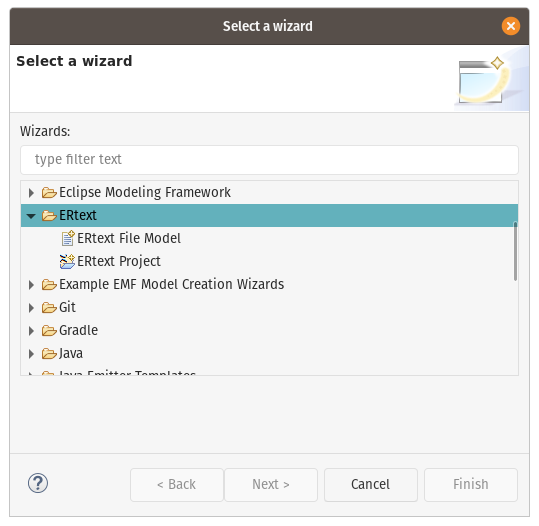
\includegraphics[width=\textwidth]{img/Wizard1.png}
    \fonte{Author.}
  \end{minipage}
  \hfill
  \begin{minipage}[b]{0.55\textwidth}
    \caption{Template proposals.}
    \label{fig:templateProposal}
    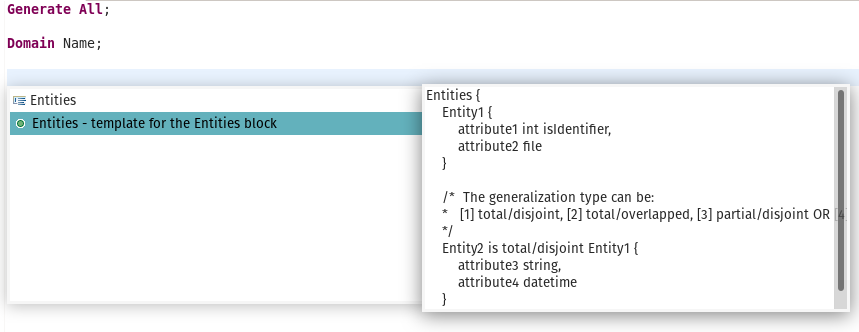
\includegraphics[width=\textwidth]{img/CodeSnippetRecomendation.png}
    \fonte{Author.}
  \end{minipage}
\end{figure}

%------------------------------------------------------------------------------
\subsection{Toy Example}
%------------------------------------------------------------------------------

% Para demonstrar um exemplo de uso vamos imaginar um modelo hipótico de uma rede social simples.
% Neste exemplo existem sete (7) entidades.
% Uma entidade Usuário, que é especializada em Pessoas e Organizações.
% Os Usuários podem compartilhar Postagens, que por sua vez podem conter Fotos associadas.
% Os usuários podem ter relacionamentos de amizade com outros usuários, bem como participar de Grupos.
% Finalmente, para cada relação de Usuários que pertencem a Grupos, nós modelamos um Papel (e.g. dono, moderador, participante, etc).
% Como a relação de Usuários pertencendo a Grupos é uma relação N:N, a adição do Papel gera uma relação ternária (associativa) entra a entidade derivada e as ocorrências de papéis.
% A descrição é exibida na Figura \ref{fig:toyExampleDSlDescription}.

To demonstrate a toy example, let's imagine a hypothetical model of a simple \texttt{social network}.
In this example, there are seven (7) entities.
A \texttt{User} entity, which specializes in the \texttt{People} and \texttt{Organization} entities.
Users can share \texttt{Posts} that may contain associated \texttt{Photos}.
Users can have friendly relationships with other users as well as participate in \texttt{Groups}.
Finally, for each relationship of Users that belong to Groups, we model \texttt{Roles} (\textit{e.g.} owner, moderator, participant, etc) entity.
As the relationship of Users belonging to Groups is an N:N relationship, the addition of Role generates a ternary (associative) relationship between the derived entity and role occurrences.
Figure \ref{fig:toyExampleDSlDescription} shows the description.

\begin{figure}[!htb]
    \centering
    \caption{Description of a social network example.}
    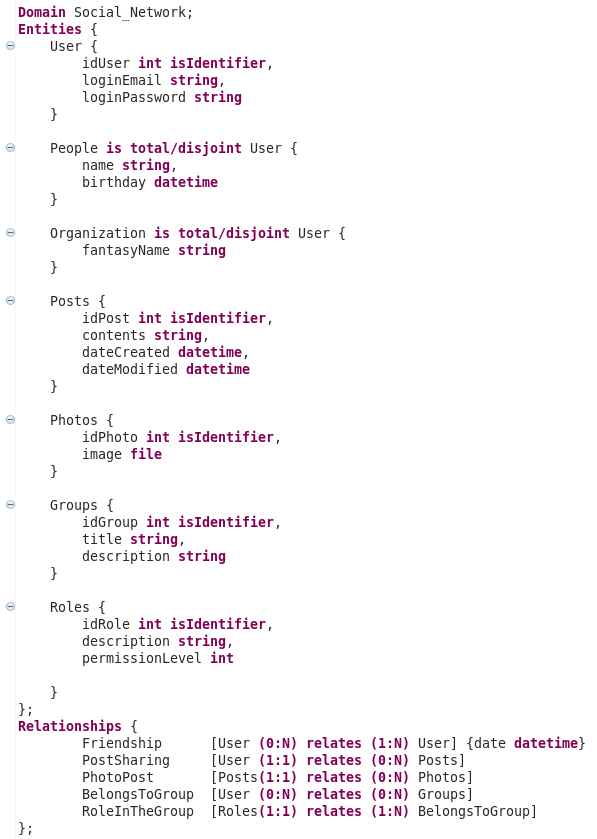
\includegraphics[width=0.5\textwidth]{img/toyExampleDSlDescription.png}
    \fonte{Author.}
    \label{fig:toyExampleDSlDescription}
\end{figure}

% Como dito anteriormente, os geradores são chamados cada vez que o modelo é salvo.
% Se o modelo for considerados válido conforme a sintaxe da \ac{dsl}, o modelo Ecore em memória é despachado para o gerador principal, que então faz um novo encaminhamento para os outros geradores especializados, gerando assim o diagrama, o modelo HTML e os arquivos SQLs.
% Nestes geradores os arquivos destino são gerados em uma pasta chamada src-gen na raiz do projeto.
As stated earlier, the tool calls the generators each time that saves the model.
% As stated earlier, the generators are called each time the model is saved.
If the tool considers the model valid according to the \ac{dsl} syntax, it dispatches the in-memory Ecore model to the main generator. Then forwards it to the other specialized generators, thus producing the diagram (conceptual model), \ac{html} (logical model), and the \ac{sql} files (physical model).
% If the model is considered valid according to the \ac{dsl} syntax, the in-memory Ecore model is dispatched to the main generator, which then forwards it to the other specialized generators, thus producing the diagram (conceptual model), \ac{html} (logical model) and the \ac{sql} files (physical model).
In these generators, the tool generates the target files in a folder called ``\texttt{src-gen}'' at the root of the project folder.


% A representação da herança entre a entidade User e as entidades People e Organization é apresentado na Figura \ref{fig:Diagram_Generalization}. 
% Ao utilizar a PlantUML a notação UML para diagramas de classe é usada.
% O equivalente gerado no modelo lógico é apresentado na Figura \ref{fig:Logical_Generalization}.
Figure \ref{fig:Diagram_Generalization} display the representation of the inheritance between the \texttt{User} entity and the \texttt{People} and \texttt{Organization} entities.
The tool uses the UML notation for class diagrams when using PlantUML.
Figure \ref{fig:Logical_Generalization} shows the equivalent generated in the logical model.
% The representation of the inheritance among the \texttt{User} entity, the \texttt{People}, and \texttt{Organization} entities is presented in Figure \ref{fig:Diagram_Generalization}.
% When using PlantUML the UML notation for class diagrams is used.
% The equivalent generated in the logical model is shown in Figure \ref{fig:Logical_Generalization}.

\begin{figure}[!htb]
  \centering
  \begin{minipage}[b]{0.4\textwidth}
    \caption{Diagram snippet of a generalization.}
    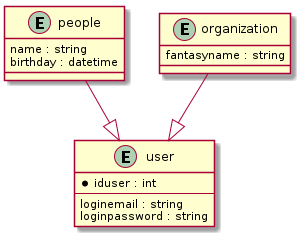
\includegraphics[width=\textwidth]{img/Diagram_Generalization.png}
    \label{fig:Diagram_Generalization}
    \fonte{Author.}
  \end{minipage}
  \hfill
  \begin{minipage}[b]{0.5\textwidth}
    \caption{Logical model snippet of a generalization.}
    \label{fig:Logical_Generalization}
    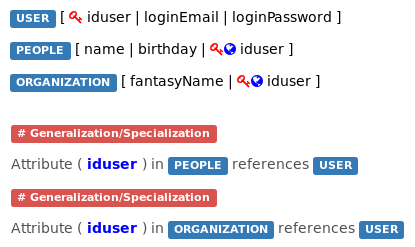
\includegraphics[width=\textwidth]{img/Logical_Generalization.png}
    \fonte{Author.}
  \end{minipage}
\end{figure}


\begin{figure}[!htb]
    \centering
    \caption{SQL model snippet for generalizations.}
    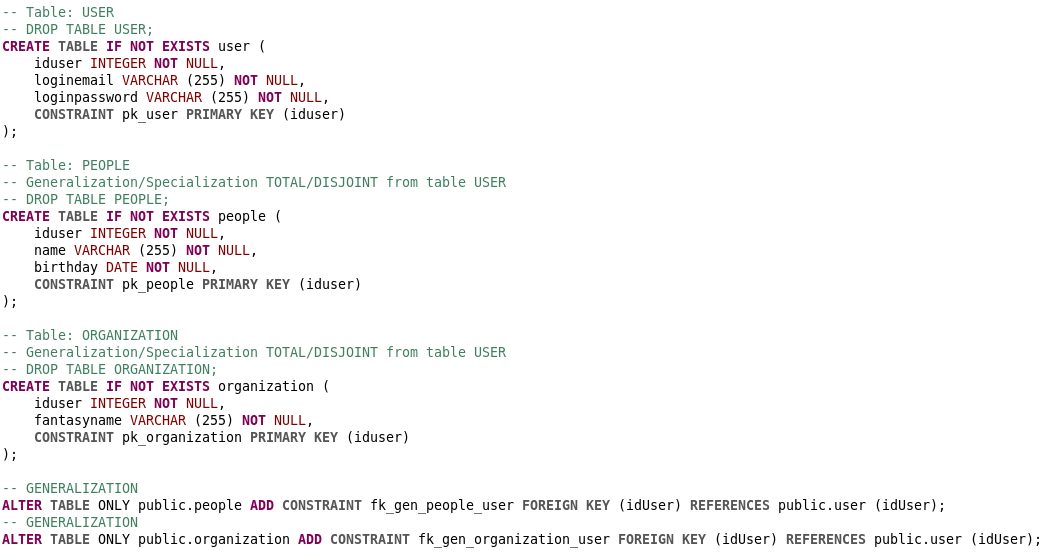
\includegraphics[width=\textwidth]{img/SQL_Generalization.png}
    \fonte{Author.}
    \label{fig:SQL_Generalization}
\end{figure}

% O modelo SQL gerado, para a plataforma PostgreSQL, também equivalente aos modelos anteriores é apresentado na Figura \ref{fig:SQL_Generalization}
Figure \ref{fig:SQL_Generalization} shows the generated SQL model for the PostgreSQL platform, also equivalent to the previous models.
% The generated SQL model, for the PostgreSQL platform, also equivalent to the previous models, is shown in Figure \ref{fig:SQL_Generalization}
% A mesma lógica é usada para relações binárias e entidades tenárias nos modelos lógicos e físicos, ou seja, as entidades são criadas com as referências sendo resolvidas (chaves estrangeiras).
% As relações tem seus mapeamentos sendo indicados logo em seguida da estrutura das entidades.
% Nas Figuras a seguir (\ref{fig:Diagram_Binary} e \ref{fig:Logical_Binary}) os modelos são apresentados com três (3) relações binárias (PostSharing, PhotoPost e FriendShip).
% No modelo conceitual a autorelação N:N Friendship da entidade User é apresentada omitindo a entidade que é derivada.
% Entretanto, no modelo lógico ela é mostrada juntamente com as outras relações, tanto em estrutura quanto nos mapeamentos detectados.
% Para conhecimento, no modelo lógico os simbolos de chave em vermelho representam as chaves primárias.
% Os símbolos de globo em azul representam as chaves estrangeiras.
% Quando um atributo é ambos os tipos de chaves, ambos os símbolos são utilizados.
% A Figura \ref{fig:SQL_Binary} apresenta o modelo \ac{sql} equivalente gerado pela ferramenta.
The same logic is used for binary relationships and ternary entities in both logical and physical models, that is, entities are created with the references being resolved (foreign keys).
The relationships have their mappings being indicated right after the structure of the entities.
In Figures \ref{fig:Diagram_Binary} and \ref{fig:Logical_Binary}, the models are presented with three (3) binary relations (PostSharing, PhotoPost, and FriendShip).
In the conceptual model the N:N Friendship self-relation of the User entity is presented omitting the entity that is derived.
However, in the logical model, it is shown together with the other relationships, both in structure and in the detected mapping list.
For knowledge, the red key symbols represent the primary keys in the logic model.
Blue globe symbols represent foreign keys.
When an attribute is both key types, both symbols are used.
Figure \ref{fig:SQL_Binary} shows the equivalent \ac{sql} model generated by the tool.

\begin{figure}[!htb]
  \centering
  \begin{minipage}[b]{0.4\textwidth}
    \caption{Diagram snippet with binary relatioships.}
    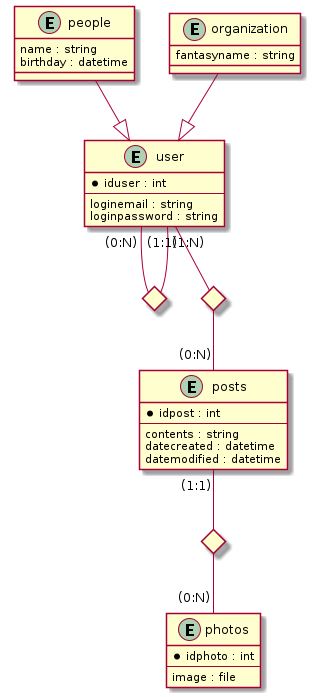
\includegraphics[width=0.8\textwidth]{img/Diagram_binary.png}
    \label{fig:Diagram_Binary}
    \fonte{Author.}
  \end{minipage}
  \hfill
  \begin{minipage}[b]{0.5\textwidth}
    \caption{Logical model snippet with binary relationships.}
    \label{fig:Logical_Binary}
    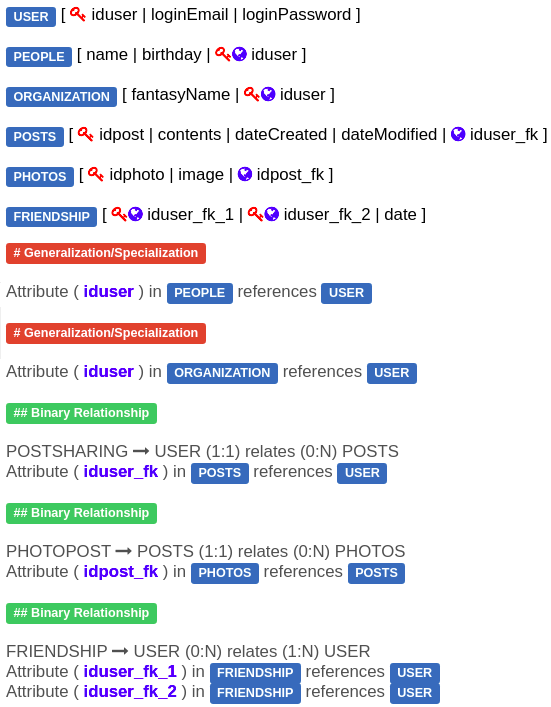
\includegraphics[width=0.8\textwidth]{img/Logical_binary.png}
    \fonte{Author.}
  \end{minipage}
\end{figure}

\begin{figure}[!htb]
    \centering
    \caption{SQL model snippet with binary relationships.}
    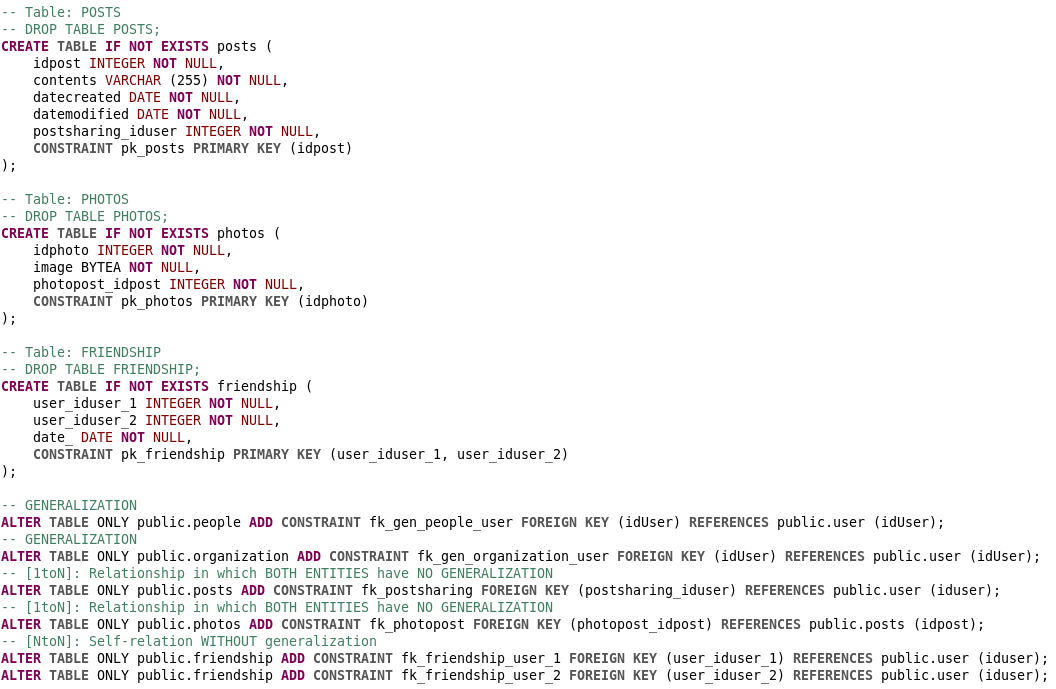
\includegraphics[width=0.85\textwidth]{img/SQL_Binary.png}
    % \fonte{Author.}
    \label{fig:SQL_Binary}
\end{figure}

% No que diz respeito as relações ternárias (associativas) quando um diagrama é gerado há a indição onde elas ocorrem na imagem com a ajuda de uma anotação.
% No modelo lógico é exibida a entidade derivada deste tipo de relação.
% Basicamente, há a associação entre uma relação N:N com outra entidade.
% Para melhor compreensão do usuário, nós mantemos o mesmo padrão de apresentação, fazendo uso de rótulos coloridos indicando o tipo de mapeamento detectado.
% As Figuras \ref{fig:Diagram_Ternary} e \ref{fig:Logical_Ternary} mostram um fragmento deste tipo específico de relação sendo mapeada na nossa ferramenta, com base no modelo descrito no ínicio desta seção.
Concerning ternary (associative) relationships, when it generates a diagram, there is an indication of where they occur in the image with the help of an annotation.
% With respect to ternary (associative) relationships, when a diagram is generated there is an indication of where they occur in the image with the help of an annotation.
In the logical model, the entity derived from this type of relationship is displayed.
Basically, there is an association between an N:N relationship with another entity.
% For better user understanding, we keep the same presentation pattern, making use of colored labels indicating the type of mapping detected.
For better user understanding, we keep the same presentation pattern using colored labels that indicate the mapping detected type.
% Figures \ref{fig:Diagram_Ternary} and \ref{fig:Logical_Ternary} show a fragment of this specific type of relationship being mapped in our tool, based on the model described at the beginning of this section.
Figures \ref{fig:Diagram_Ternary} and \ref{fig:Logical_Ternary} show a fragment of this specific relationship type mapped in our tool based on the model described at the beginning of this section.

\begin{figure}[!htb]
  \centering
  \begin{minipage}[b]{0.4\textwidth}
    \caption{Diagram snippet with a ternary relationship.}
    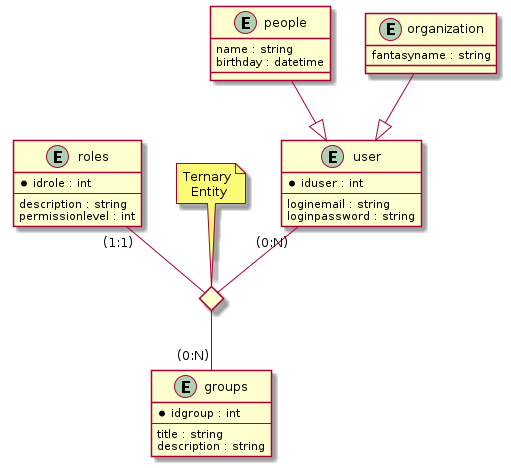
\includegraphics[width=\textwidth]{img/Diagram_Ternary.png}
    \label{fig:Diagram_Ternary}
    \fonte{Author.}
  \end{minipage}
  \hfill
  \begin{minipage}[b]{0.5\textwidth}
    \caption{Logical model snippet with a ternary relationship.}
    \label{fig:Logical_Ternary}
    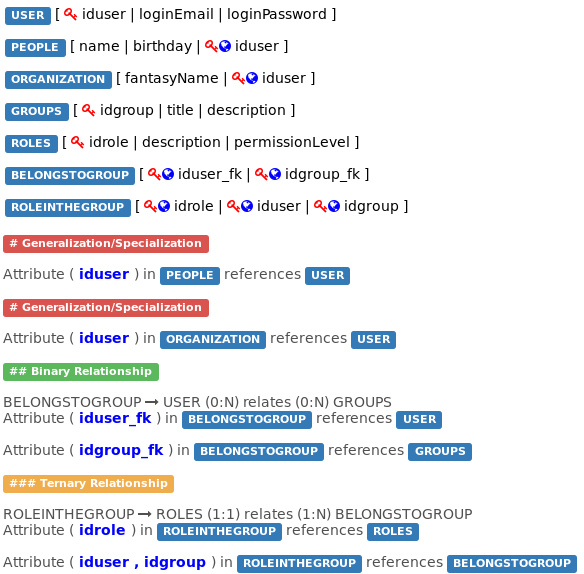
\includegraphics[width=0.8\textwidth]{img/Logical_Ternary.png}
    \fonte{Author.}
  \end{minipage}
\end{figure}

\begin{figure}[!htb]
    \centering
    \caption{SQL model snippet with a ternary relationship.}
    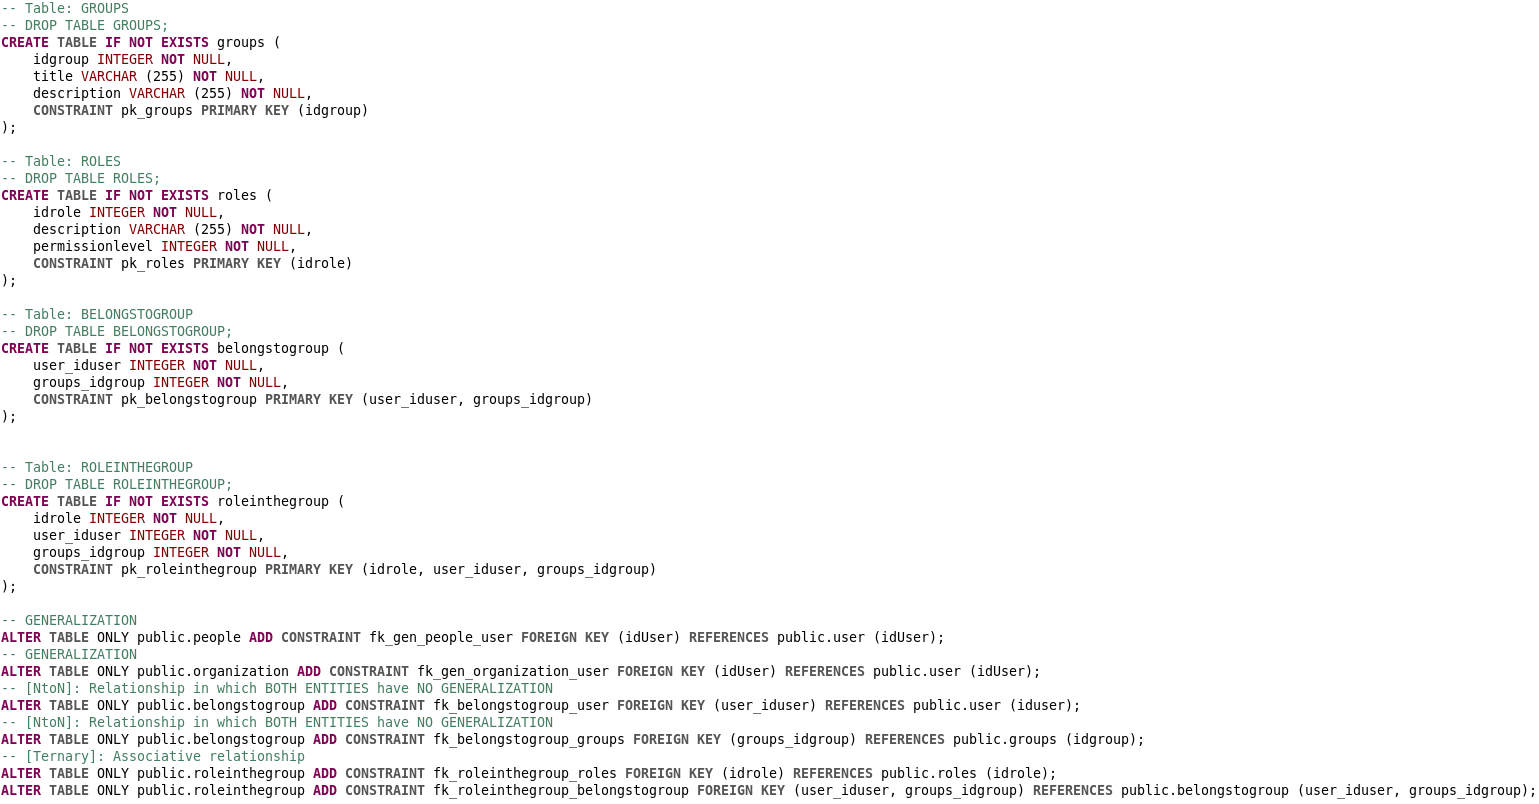
\includegraphics[width=\textwidth]{img/SQL_Ternary.png}
    \fonte{Author.}
    \label{fig:SQL_Ternary}
\end{figure}


% Finalmente, o mapeamento para o arquivo \ac{sql} apresentado na Figura \ref{fig:SQL_Ternary} segue também o mesmo padrão, gerando os comandos \texttt{Alter Table} após a definição da estrutura das entidades.
% Algo que é importante de se relatar é que inicialmente os modelos \ac{sql} estavam sendo criados com as restriçoes chaves estrangeiras sendo declaradas já no corpo das tabelas.
% Isso foi feito por acreditarmos que a legibilidade e compreensão das \ac{ddl} era facilitada.
% Contudo, foi necessário um reavaliação desta estratégia uma vez que os códigos \ac{sql} gerados não estavam sendo executados nas plataformas alvo.
% Isso acontecia pois se tornou díficil prever quando uma restrição indicava relação com algum atributo de entidade ainda não criada.
% Tentou-se implementar formas de se fazer a geração da ordem correta mas por conta da complexidade que se apresentou aderimos a criação das restrições via comandos \texttt{Alter Table} no final do arquivo, assim os tornando executáveis nos \ac{rdms}.
Finally, Figure \ref{fig:SQL_Ternary} shows the mapping to the \ac{sql} file also follows the same pattern, generating the \texttt{Alter Table} commands after defining the structure of the entities.
Something relevant to report is that firstly the \ac{sql} models were being created with the foreign key constraints being declared already in the bodies of the tables.
It was done because we believed that facilitates the readability and the understanding of \ac{ddl}.
% This was done because we believed that the readability and understanding of \ac{ddl} were facilitated.
However, it was necessary to re-evaluate this strategy since the generated \ac{sql} codes were not being executed successfully on the target platforms.
This happened because it became difficult to predict when a restriction indicated a relationship with some attribute of an entity not yet created.
We tried to implement ways to generate the correct order, despite due to the complexity that presented itself, we adhered to the creation of restrictions via \texttt{Alter Table} commands at the end of the file, thus making them executable in the \acp{dbms}.
% We tried to implement ways to generate the correct order, but due to the complexity that presented itself, we adhered to the creation of restrictions via \texttt{Alter Table} commands at the end of the file, thus making them executable in the \acp{dbms}.

%------------------------------------------------------------------------------
\section{Chapter Lessons}
%------------------------------------------------------------------------------
 
% Neste capítulo foram expostos os requisitos, as decisões de projeto e a arquitetura da \ac{dsl} proposta para a solução desenvolvida. 
% Também é apresentada uma visão geral da versão estável que será testada na última avaliação experimental, bem como um exemplo de uso foi descrito, com os respectivos artefatos produzidos pelos geradores sendo exibidos.
In this chapter, we have laid out the requirements, design decisions, and architecture for the developed solution.
We also presented an overview of the stable version that was tested in subsequent experimental evaluations.
Furthermore, we described an example of use with the respective artifacts produced by the generators.
% In this chapter, the requirements, design decisions and architecture of the \ac{dsl} proposal for the developed solution were exposed.
% An overview of the stable version that will be tested in the last experimental evaluation is also presented, as well as an example of use was described, with the respective artifacts produced by the generators being displayed.

% Novamente reforçamos a importância da comunidade Xtext formada por um grupo de desenvolvedores que ajudaram direta e indiretamente na implementação de grande parte da ferramenta apresentada.
% Através das interações com estes desenvolvedores houve um amadurecimento da nossa proposta, bem como nós adquirimos uma gama de habilidades técnicas e pessoais (habilidades soft e hard) que auxiliaram decisivamente no processo de otimização da DSL e do código de infraestrutura fornecida pelo framework.
Again, we reinforce the importance of the Xtext community formed by a group of developers who helped, directly and indirectly, the implementation of a large part of the presented tool.
Through interactions with these developers, our proposal matured,  even as we acquired a range of technical and personal skills (soft and hard skills) that decisively helped in the optimization process of the \ac{dsl} and the infrastructure code provided by the framework.

% Esperamos que a ferramenta de modelagem desenvolvida possa colaborar com o processo de ensino-aprendizagem, fornecendo uma gramática de fácil compreensão e uma facilidade de uso facilitado pela integração com a IDE Eclipse. 
% Finalmente, para que este objetivo seja alcançado, é imprescindível que a avaliação experimental seja devidamente planeada, executada e analisada tendo em conta as funcionalidades que nos propomos oferecer.
We hope that the developed modeling tool can collaborate with the teaching-learning process, providing an easy-to-understand grammar and ease of use facilitated by the Eclipse \ac{ide} integration.
% We hope that the developed modeling tool can collaborate with the teaching-learning process, providing an easy-to-understand grammar and ease of use facilitated by the integration with the Eclipse \ac{ide}.
Finally, to achieve this objective, the experimental evaluations were duly planned, executed and analyzed, taking into account the characteristics that we proposed to offer.
% Finally, in order to achieve this goal, it is imperative that the experimental evaluation be properly planned, executed, and analyzed taking into account the features that we propose to offer.


